% Options for packages loaded elsewhere
\PassOptionsToPackage{unicode}{hyperref}
\PassOptionsToPackage{hyphens}{url}
%
\documentclass[
  french,
]{book}
\usepackage{lmodern}
\usepackage{amssymb,amsmath}
\usepackage{ifxetex,ifluatex}
\ifnum 0\ifxetex 1\fi\ifluatex 1\fi=0 % if pdftex
  \usepackage[T1]{fontenc}
  \usepackage[utf8]{inputenc}
  \usepackage{textcomp} % provide euro and other symbols
\else % if luatex or xetex
  \usepackage{unicode-math}
  \defaultfontfeatures{Scale=MatchLowercase}
  \defaultfontfeatures[\rmfamily]{Ligatures=TeX,Scale=1}
\fi
% Use upquote if available, for straight quotes in verbatim environments
\IfFileExists{upquote.sty}{\usepackage{upquote}}{}
\IfFileExists{microtype.sty}{% use microtype if available
  \usepackage[]{microtype}
  \UseMicrotypeSet[protrusion]{basicmath} % disable protrusion for tt fonts
}{}
\makeatletter
\@ifundefined{KOMAClassName}{% if non-KOMA class
  \IfFileExists{parskip.sty}{%
    \usepackage{parskip}
  }{% else
    \setlength{\parindent}{0pt}
    \setlength{\parskip}{6pt plus 2pt minus 1pt}}
}{% if KOMA class
  \KOMAoptions{parskip=half}}
\makeatother
\usepackage{xcolor}
\IfFileExists{xurl.sty}{\usepackage{xurl}}{} % add URL line breaks if available
\IfFileExists{bookmark.sty}{\usepackage{bookmark}}{\usepackage{hyperref}}
\hypersetup{
  pdftitle={Aide-mémoire : Analyses de données \& Cartographie sur R},
  pdfauthor={Alexis Mérot},
  pdflang={fr-FR},
  hidelinks,
  pdfcreator={LaTeX via pandoc}}
\urlstyle{same} % disable monospaced font for URLs
\usepackage{color}
\usepackage{fancyvrb}
\newcommand{\VerbBar}{|}
\newcommand{\VERB}{\Verb[commandchars=\\\{\}]}
\DefineVerbatimEnvironment{Highlighting}{Verbatim}{commandchars=\\\{\}}
% Add ',fontsize=\small' for more characters per line
\usepackage{framed}
\definecolor{shadecolor}{RGB}{248,248,248}
\newenvironment{Shaded}{\begin{snugshade}}{\end{snugshade}}
\newcommand{\AlertTok}[1]{\textcolor[rgb]{0.94,0.16,0.16}{#1}}
\newcommand{\AnnotationTok}[1]{\textcolor[rgb]{0.56,0.35,0.01}{\textbf{\textit{#1}}}}
\newcommand{\AttributeTok}[1]{\textcolor[rgb]{0.77,0.63,0.00}{#1}}
\newcommand{\BaseNTok}[1]{\textcolor[rgb]{0.00,0.00,0.81}{#1}}
\newcommand{\BuiltInTok}[1]{#1}
\newcommand{\CharTok}[1]{\textcolor[rgb]{0.31,0.60,0.02}{#1}}
\newcommand{\CommentTok}[1]{\textcolor[rgb]{0.56,0.35,0.01}{\textit{#1}}}
\newcommand{\CommentVarTok}[1]{\textcolor[rgb]{0.56,0.35,0.01}{\textbf{\textit{#1}}}}
\newcommand{\ConstantTok}[1]{\textcolor[rgb]{0.00,0.00,0.00}{#1}}
\newcommand{\ControlFlowTok}[1]{\textcolor[rgb]{0.13,0.29,0.53}{\textbf{#1}}}
\newcommand{\DataTypeTok}[1]{\textcolor[rgb]{0.13,0.29,0.53}{#1}}
\newcommand{\DecValTok}[1]{\textcolor[rgb]{0.00,0.00,0.81}{#1}}
\newcommand{\DocumentationTok}[1]{\textcolor[rgb]{0.56,0.35,0.01}{\textbf{\textit{#1}}}}
\newcommand{\ErrorTok}[1]{\textcolor[rgb]{0.64,0.00,0.00}{\textbf{#1}}}
\newcommand{\ExtensionTok}[1]{#1}
\newcommand{\FloatTok}[1]{\textcolor[rgb]{0.00,0.00,0.81}{#1}}
\newcommand{\FunctionTok}[1]{\textcolor[rgb]{0.00,0.00,0.00}{#1}}
\newcommand{\ImportTok}[1]{#1}
\newcommand{\InformationTok}[1]{\textcolor[rgb]{0.56,0.35,0.01}{\textbf{\textit{#1}}}}
\newcommand{\KeywordTok}[1]{\textcolor[rgb]{0.13,0.29,0.53}{\textbf{#1}}}
\newcommand{\NormalTok}[1]{#1}
\newcommand{\OperatorTok}[1]{\textcolor[rgb]{0.81,0.36,0.00}{\textbf{#1}}}
\newcommand{\OtherTok}[1]{\textcolor[rgb]{0.56,0.35,0.01}{#1}}
\newcommand{\PreprocessorTok}[1]{\textcolor[rgb]{0.56,0.35,0.01}{\textit{#1}}}
\newcommand{\RegionMarkerTok}[1]{#1}
\newcommand{\SpecialCharTok}[1]{\textcolor[rgb]{0.00,0.00,0.00}{#1}}
\newcommand{\SpecialStringTok}[1]{\textcolor[rgb]{0.31,0.60,0.02}{#1}}
\newcommand{\StringTok}[1]{\textcolor[rgb]{0.31,0.60,0.02}{#1}}
\newcommand{\VariableTok}[1]{\textcolor[rgb]{0.00,0.00,0.00}{#1}}
\newcommand{\VerbatimStringTok}[1]{\textcolor[rgb]{0.31,0.60,0.02}{#1}}
\newcommand{\WarningTok}[1]{\textcolor[rgb]{0.56,0.35,0.01}{\textbf{\textit{#1}}}}
\usepackage{longtable,booktabs}
% Correct order of tables after \paragraph or \subparagraph
\usepackage{etoolbox}
\makeatletter
\patchcmd\longtable{\par}{\if@noskipsec\mbox{}\fi\par}{}{}
\makeatother
% Allow footnotes in longtable head/foot
\IfFileExists{footnotehyper.sty}{\usepackage{footnotehyper}}{\usepackage{footnote}}
\makesavenoteenv{longtable}
\usepackage{graphicx}
\makeatletter
\def\maxwidth{\ifdim\Gin@nat@width>\linewidth\linewidth\else\Gin@nat@width\fi}
\def\maxheight{\ifdim\Gin@nat@height>\textheight\textheight\else\Gin@nat@height\fi}
\makeatother
% Scale images if necessary, so that they will not overflow the page
% margins by default, and it is still possible to overwrite the defaults
% using explicit options in \includegraphics[width, height, ...]{}
\setkeys{Gin}{width=\maxwidth,height=\maxheight,keepaspectratio}
% Set default figure placement to htbp
\makeatletter
\def\fps@figure{htbp}
\makeatother
\setlength{\emergencystretch}{3em} % prevent overfull lines
\providecommand{\tightlist}{%
  \setlength{\itemsep}{0pt}\setlength{\parskip}{0pt}}
\setcounter{secnumdepth}{5}
\usepackage{booktabs}
\usepackage{csquotes}
\usepackage[french]{babel} % Ajout du français
\usepackage{tcolorbox}

\newtcolorbox{blackbox}{
  colback=black!5!white,
  colframe=orange,
  coltext=black,
  boxsep=5pt,
  arc=4pt}

\newenvironment{infobox}[1]
  {
  \begin{itemize}
  \renewcommand{\labelitemi}{
    \raisebox{-.7\height}[0pt][0pt]{
      {\setkeys{Gin}{width=3em,keepaspectratio}
        \includegraphics{images/#1}}
    }
  }
  \setlength{\fboxsep}{1em}
  \begin{blackbox}
  \item
  }
  {
  \end{blackbox}
  \end{itemize}
  }
\ifxetex
  % Load polyglossia as late as possible: uses bidi with RTL langages (e.g. Hebrew, Arabic)
  \usepackage{polyglossia}
  \setmainlanguage[]{french}
\else
  \usepackage[shorthands=off,main=french]{babel}
\fi
\ifluatex
  \usepackage{selnolig}  % disable illegal ligatures
\fi
\usepackage[]{natbib}
\bibliographystyle{apalike}

\title{Aide-mémoire : Analyses de données \& Cartographie sur R}
\author{Alexis Mérot}
\date{Modifié le : 2020-08-13}

\begin{document}
\maketitle

{
\setcounter{tocdepth}{1}
\tableofcontents
}
\hypertarget{introduction}{%
\chapter*{Introduction}\label{introduction}}
\addcontentsline{toc}{chapter}{Introduction}

\begin{infobox}{caution}

Cet aide-mémoire n'est pour l'instant qu'un brouillon. Il est donc loin d'être complet et l'écriture est pour l'instant très succincte.

\end{infobox}

Ce projet est un ensemble de notes écrites en R Markdown \citep{R-rmarkdown} et via
le package \texttt{bookdown} (\url{https://github.com/rstudio/bookdown}). Ces notes
s'accumuleront au fur et à mesure de mon apprentissage des différents outils et
concepts dont j'ai besoin pour les analyses de données et la programmation. Cela
me permet de les comprendre, les mémoriser, ainsi que de les partager.

L'aide-mémoire s'insérera peut-être dans un autre plus gros projet : la création
d'un blog répertoriant tous mes projets et mon CV. Il commencera certainement
lorsque je pourrai démarrer la lecture de la documentation de l'excellent
package \texttt{blogdown} (\url{https://bookdown.org/yihui/blogdown/}).

Cet aide-mémoire intégrera les notions théoriques indispensables en statistique
et en cartographie, ainsi que les outils proposés par R (et si besoin d'autres
langages) pour la mise en pratique à travers d'exemples. Étant principalement
intéressé par la Biologie de la conservation et globalement l'Écologie, les
exemples se focaliseront pour la plupart sur des données en lien à ces domaines.

Toutes les sources qui m'ont été utiles pour acquérir ces connaissances seront
accessibles dans les références bibliographiques ou dans les ressources Internet
à la fin des chapitres.

Il n'y a pour l'instant qu'une version en ligne, mais une version PDF sera aussi disponible en téléchargement lorsque l'aide-mémoire sera plus mature.

\hypertarget{rmarkdown}{%
\chapter{R Markdown, Bookdown \& Blogdown}\label{rmarkdown}}

\begin{infobox}{caution}

\textbf{Work In Progress}

\end{infobox}

\hypertarget{pourquoi-rmarkdown}{%
\section{Pourquoi R Markdown ?}\label{pourquoi-rmarkdown}}

R Markdown désigne un format de fichier (à l'extension \textbf{.Rmd}) et plus
globalement le framework utilisé pour créer plus facilement des documents
(généralement scientifiques) automatisés. Ces documents peuvent ainsi être
totalement reproductibles et plusieurs formats de rendu final (statiques ou
dynamiques) sont supportés.

Le fichier est écrit via le langage Markdown et des sections de code R peuvent y
être insérées facilement (ainsi que du code écrit via d'autres langages tels
que Python ou SQL). Cela offre une syntaxe facile à lire et à écrire tout en
permettant de générer un document structuré et élégant.

Pour que cela fonctionne, R Markdown est lié à deux packages : \texttt{knitr} et le
convertisseur universel de document \texttt{pandoc} (Fig. \ref{fig:rmarkdownflow}).\\
Le package \texttt{knitr} permet la création, à partir du fichier \textbf{.Rmd}, d'un fichier
au format \textbf{md} contenant le code et sa sortie. Ce fichier est alors converti
dans le format de rendu final voulu via \texttt{pandoc} (\textbf{.html}, \textbf{.pdf}, etc).



\begin{figure}

{\centering 
\includegraphics[width=0.6\linewidth]{images/rmarkdownflow} 

}

\caption{\emph{Source : \url{https://rmarkdown.rstudio.com/lesson-2.html}}}\label{fig:rmarkdownflow}
\end{figure}

Toutes mes notes seront donc écrites via R Markdown, et cette section intégrera
toutes les astuces intéressantes que je rencontre au fur et à mesure des
besoins.

Pour ne pas paraphraser tout l'excellent guide de \citet{rmarkdown2018}, je vous invite à
lire leur excellent guide gratuit : \url{https://bookdown.org/yihui/rmarkdown/},
ainsi que le livre en cours d'écriture
\href{https://bookdown.org/yihui/rmarkdown-cookbook/}{R Markdown Cookbook}.

\begin{center}\rule{0.5\linewidth}{0.5pt}\end{center}

\hypertarget{ref-rmd}{%
\section*{Liste de ressources Internet utiles}\label{ref-rmd}}
\addcontentsline{toc}{section}{Liste de ressources Internet utiles}

\begin{itemize}
\tightlist
\item
  R Markdown :

  \begin{itemize}
  \tightlist
  \item
    \href{https://rmarkdown.rstudio.com/lesson-1.html}{Vue d'ensemble} de R Markdown
  \item
    \href{https://ysc-rmarkdown.netlify.app/}{Cours} sur la communication avec R Markdown
  \item
    \href{https://emilyriederer.netlify.app/post/rmarkdown-driven-development/}{Comment utiliser R Markdown}
    comme base pour le développement de packages bien organisés
  \item
    Quelques \href{https://www.dataquest.io/blog/r-markdown-tips-tricks-and-shortcuts/}{trucs et astuces}
    sur R Markdown
  \item
    \href{https://holtzy.github.io/Pimp-my-rmd/}{Comment donner du \emph{peps}}
    à mon document RMD
  \item
    \href{https://www.dataquest.io/blog/r-markdown-guide-cheatsheet/}{Un autre guide}
    de R Markdown
  \item
    \href{https://bookdown.org/yihui/rmarkdown/}{Guide complet} de R Markdown
  \item
    \href{https://bookdown.org/yihui/rmarkdown-cookbook/}{Nouveau guide}
    de R Markdown (\textbf{\emph{en cours d'écriture}})
  \item
    \href{https://danawanzer.com/using-r-for-immediate-reporting-in-evaluation/}{Création d'un template}
    R Markdown
  \end{itemize}
\item
  Bookdown :

  \begin{itemize}
  \tightlist
  \item
    \href{https://bookdown.org/home/about/}{Site officiel} de \texttt{bookdown}
  \item
    \href{https://bookdown.org/yihui/bookdown/}{Guide complet} de \texttt{bookdown}
  \item
    Extension à \texttt{bookdown} : \href{https://bookdown.org/baydap/bookdownplus/}{\texttt{bookdownplus}}
  \item
    \href{https://statistique-et-logiciel-r.com/creer-un-livre-document-avec-bookdown/}{Guide en français}
    de \texttt{bookdown}
  \item
    \href{https://thinkr.fr/rediger-avec-bookdown-pourquoi-comment/}{Introduction en français}
    à \texttt{bookdown}
  \end{itemize}
\item
  Blogdown :

  \begin{itemize}
  \tightlist
  \item
    \href{https://bookdown.org/yihui/blogdown/}{Guide complet} sur \texttt{blogdown}
  \end{itemize}
\item
  Court \href{https://slides.yihui.org/2017-rmarkdown-UNL-Yihui-Xie.html\#1}{tutoriel}
  d'introduction sur R Markdown, \texttt{bookdown} et \texttt{blogdown}
\item
  Guide pour le package \href{https://yihui.org/knitr/}{\texttt{knitr}}
\item
  \href{https://yihui.org/knitr/options/}{Options} valables pour les \emph{chunks} de code
  et le package \texttt{knitr}
\end{itemize}

\begin{center}\rule{0.5\linewidth}{0.5pt}\end{center}

\hypertarget{data-analysis}{%
\chapter{Extraction/importation, nettoyage \& manipulation des données}\label{data-analysis}}

\begin{infobox}{caution}

\textbf{Work In Progress}

\end{infobox}

\hypertarget{extraction-de-donnuxe9es-provenant-dun-pdf}{%
\section{Extraction de données provenant d'un PDF}\label{extraction-de-donnuxe9es-provenant-dun-pdf}}

\hypertarget{ruxe9cupuxe9ration-de-donnuxe9es-provenant-du-web-le-web-scraping}{%
\section{\texorpdfstring{Récupération de données provenant du web : le \emph{web scraping}}{Récupération de données provenant du web : le web scraping}}\label{ruxe9cupuxe9ration-de-donnuxe9es-provenant-du-web-le-web-scraping}}

\hypertarget{ref-data-analysis}{%
\section*{Liste de ressources Internet utiles}\label{ref-data-analysis}}
\addcontentsline{toc}{section}{Liste de ressources Internet utiles}

\hypertarget{statistique}{%
\chapter{Statistique}\label{statistique}}

\begin{infobox}{caution}

\textbf{Work In Progress}

\end{infobox}

\hypertarget{quelques-notions-cluxe9s}{%
\section{Quelques notions clés}\label{quelques-notions-cluxe9s}}

Concepts à comprendre :

\begin{itemize}
\tightlist
\item
  Théorie des probabilités
\item
  Variable aléatoire réelle
\item
  Fonction de répartition (ou fonction de distribution cumulative) d'une
  variable aléatoire
\item
  Fonction de densité ou densité de probabilité
\end{itemize}

\hypertarget{frequentiste}{%
\section{Statistique fréquentiste}\label{frequentiste}}

\begin{center}\rule{0.5\linewidth}{0.5pt}\end{center}

\hypertarget{ref-stat-freq}{%
\section*{Liste de ressources Internet utiles}\label{ref-stat-freq}}
\addcontentsline{toc}{section}{Liste de ressources Internet utiles}

\begin{center}\rule{0.5\linewidth}{0.5pt}\end{center}

\hypertarget{bayesienne}{%
\section{Statistique bayésienne}\label{bayesienne}}

\begin{center}\rule{0.5\linewidth}{0.5pt}\end{center}

\hypertarget{ref-stat-bayes}{%
\section*{Liste de ressources Internet utiles}\label{ref-stat-bayes}}
\addcontentsline{toc}{section}{Liste de ressources Internet utiles}

\begin{center}\rule{0.5\linewidth}{0.5pt}\end{center}

\hypertarget{dataviz}{%
\chapter{\texorpdfstring{Visualisation des données : la \emph{Dataviz}}{Visualisation des données : la Dataviz}}\label{dataviz}}

\begin{infobox}{caution}

\textbf{Work In Progress}

\end{infobox}

\hypertarget{SIG}{%
\chapter{Systèmes d'Information Géographique \& Cartographie}\label{SIG}}

\begin{infobox}{caution}

\textbf{Work In Progress}

\end{infobox}

\hypertarget{whatis-sig}{%
\section{Qu'est-ce qu'un SIG ?}\label{whatis-sig}}

Un Système d'Information Géographique est, comme tout Système d'Information
\footnote{Cf. le cours sur
  \href{https://openclassrooms.com/fr/courses/2100086-decouvrez-le-monde-des-systemes-dinformation}{Openclassroom}.}, un ensemble organisé de ressources ayant pour fonction de collecter,
stocker, traiter et diffuser des informations \footnote{Cf. la page Wikipédia sur le
  \href{https://fr.wikipedia.org/wiki/Syst\%C3\%A8me_d\%27information_g\%C3\%A9ographique}{Système d'Information Géographique}.}. Ici, ces informations
(généralement informatisées) sont des données géospatiales stockées sous forme
de couches d'informations superposées et reliées les unes aux autres par un
référentiel cartographique \footnote{Fond de carte représentant un territoire géographique sur lequel
  peuvent venir s'insérer de nouvelles données cartographiques.}. Les SIG sont devenus des outils
essentiels dans de nombreux domaines tels que l'écologie, la médecine ou la
sociologie.

Pour aider les utilisateurs au traitement des données géospatiales, il existe de
performants et très utilisés logiciels gratuits ou payants tels que
\href{https://www.qgis.org/fr/site/}{QGis} ou
\href{https://www.arcgis.com/index.html}{ArcGIS}. Ces logiciels offrent une approche
graphique à la lecture, l'écriture, la manipulation et la visualisation des
données. Ceci peut néanmoins limiter la reproductibilité et l'automatisation des
projets. Pour remédier à cela, de nombreux langages de programmation peuvent
être utilisés pour écrire et partager des scripts. Parmi les plus utilisés, il y
a \href{https://www.python.org/}{Python} (qui est notamment utilisé pour la
conception de plugins dans les logiciels de SIG) et
\href{https://www.r-project.org/about.html}{R} (dont les scripts sont maintenant
exécutables dans QGis). En plus de cela, l'approche en lignes de commande permet
de se libérer de certaines contraintes imposées par ces logiciels ainsi que
d'avoir plus de contrôle sur ce que l'ont fait (même si ces logiciels sont de
plus en plus performants).

\hypertarget{R-sig}{%
\section{R en tant que SIG}\label{R-sig}}

Afin d'avoir un bon aperçu et une bonne base sur l'utilisation de R en tant que
SIG, je vous invite à lire le livre \emph{Geocomputation with R} de \citet{geocomputation}.
Ce livre est mis à jour régulièrement et consultable gratuitement à cette
adresse : \url{https://geocompr.robinlovelace.net/}. Si vous préférez le format
papier et/ou voulez soutenir les auteurs, il est bien sûr disponible à l'achat.

Ayant commencé à apprendre les analyses statistiques avec R, c'est naturellement
que je me suis tourné vers ce langage pour la cartographie et l'analyse des
données géospatiales. En effet, la communauté de R a créé de performants et
magnifiques packages de cartographie et de géocalcul libres, gratuits et bien
documentés. Je m'intéresserai donc de plus près à ce qu'offre par exemple Python
lorsque j'aurai maîtrisé suffisamment R. Un autre langage élégant et très récent
qui est à regarder de très près est \href{https://julialang.org/}{Julia}, qui offrira
certainement des packages rapides et performants au fur et à mesure de sa
maturité. Par ailleurs, même si des programmes manqueraient à R ou si d'autres
langages possèdent des programmes plus adaptés pour certaines tâches, des
packages R offrent la possibilité d'en faciliter l'accès. Par exemple, les
packages tels que \href{https://github.com/RcppCore/Rcpp}{\texttt{Rcpp}} et
\href{https://rstudio.github.io/reticulate/}{\texttt{Reticulate}} permettent l'utilisation
de programmes écrits respectivement en C++ et Python.

D'autres caractéristiques intéressantes de R sont sa flexibilité et sa constante
évolution. Par exemple, il offre maintenant la possibilité de faire facilement
des applications web et des cartes interactives notamment via les packages
\href{https://shiny.rstudio.com/}{\texttt{Shiny}} et
\href{https://rstudio.github.io/leaflet/}{\texttt{Leaflet}}. Il offre par la même occasion
divers outils d'analyses avancées, de modélisation et de visualisation qui sont
mis à jour et améliorés régulièrement.

Pour plus d'informations concernant les atouts de R en tant que SIG ainsi qu'un
bref aperçu de l'utilité des autres langages tels que Python, Java et C++, je
vous invite à lire le chapitre \href{https://geocompr.robinlovelace.net/intro.html\#why-use-r-for-geocomputation}{Why use R for
geocomputation}
du livre de \citet{geocomputation}.

\hypertarget{data-sig}{%
\section{\texorpdfstring{La représentation des données : les \emph{vecteurs} et les \emph{rasters}}{La représentation des données : les vecteurs et les rasters}}\label{data-sig}}

Pour représenter numériquement les données spatiales, deux modèles de base sont
utilisés : les \emph{vecteurs} (mode vectoriel) et les \emph{rasters} (mode matriciel).
L'une des principales différences entre ces deux modèles est qu'un vecteur est
un \emph{objet} (ou entité) tandis que le raster est une \emph{image}. Ainsi, les vecteurs
sont constitués de points, de lignes et de polygones créés à partir d'équations
mathématiques, tandis que les rasters sont des grilles constituées de cellules
de même taille (les pixels). C'est cette différence qui fait que les vecteurs ne
perdent pas en netteté lorsque l'on zoome dessus, tandis que les images
(rasters) deviennent floues (elles « pixelisent »). Par ailleurs, la différence
dans la manière de stocker ces deux modèles fait que les fichiers liés aux
vecteurs ont une taille bien inférieure que ceux liés aux raster.\\
Sous R, les vecteurs et les rasters sont travaillés respectivement avec les
packages \texttt{sf} et \texttt{raster}.

\hypertarget{vectors}{%
\subsection{Les vecteurs}\label{vectors}}

Un vecteur est une image vectorielle ou dessin mathématique constitué de deux
composantes : une \textbf{composante attributaire} permettant de l'identifier, et une
\textbf{composante graphique} décrivant sa géométrie. Il est localisé grâce à un
Système de Coordonnées de Référence (ou CRS pour \emph{Coordinate Reference System}
en anglais). Les vecteurs sont basiquement composés de nœuds ou sommets qui sont
des \textbf{points dans l'espace}. À partir de ces sommets, des \textbf{formules
mathématiques} sont appliquées pour créer des \textbf{formes géométriques}. S'il n'y
a qu'un sommet, le vecteur est simplement un point. S'il y a plusieurs sommets
et que les liaisons ne forment pas une forme géométrique fermée, alors cela
forme une ligne. Si la forme est fermée, le vecteur est un polygone. La
géométrie des points est généralement en deux dimensions (\(x =\) longitude, \(y =\)
latitude), mais peut être parfois en trois dimensions si une valeur \(z\)
additionnelle est ajoutée (notamment pour représenter la hauteur au-dessus du
niveau de la mer).\\
Les vecteurs permettent donc de représenter des \textbf{données discrètes} avec des
\textbf{formes bien définies dans l'espace}.

Pour stocker la géométrie de ces \textbf{entités géographiques},
l'OGC \footnote{L'OGC est un consortium international qui développe des standards ouverts
  (OpenGIS) dans les domaines de la géomatique et de l'information géographique.} (\href{https://www.ogc.org/}{\emph{Open Geospatial Consortium}}) a développé
un modèle standardisé pour les Bases de Données Spatiales (BDS). Ce modèle
s'appelle \textbf{Modèle d'Entité Simple} (SFA pour \href{https://www.ogc.org/standards/sfa}{\emph{Simple Feature
Access}} en anglais) et permet de définir des
fonctions pour accéder, faire des calculs et construire les données, dans le but
de représenter les objets dans la réalité. C'est un modèle de données très
largement supporté dans la plupart des logiciels SIG (dont QGIS) et a
l'avantage de rendre le travail totalement transférable d'un projet à un autre
grâce à une architecture commune.

Pour amener ce modèle dans R, le package \texttt{sf} a ainsi été créé pour succéder au
package \texttt{sp} sur le long terme \footnote{Cf. la \href{https://r-spatial.github.io/sf/articles/sf1.html}{vignette}
  du package \texttt{sf} parlant de ce sujet.}. Les différents \textbf{types de
géométrie} définis par la norme standardisée de l'OGC sont donc inclus dans ce
package (fig.~\ref{fig:sfclasses}). Ces types de géométrie permettent de créer
les entités, qui sont la \textbf{représentation d'un objet dans le monde réel} (comme
un bâtiment, un champ ou un arbre). Chaque entité peut alors faire partie par
exemple du type \texttt{POINT}, \texttt{POLYLIGNE} (\texttt{LINESTRING}) ou \texttt{POLYGONE}. En plus de
cela, il est possible de créer d'autres entités à partir de l'agrégation de ces
entités basiques (formant des \texttt{MULITPOINTS}, des \texttt{MULTIPOLYLIGNES} et des
\texttt{MULTIPOLYGONES}). Une seule entité contenant plusieurs types de géométrie
différents est alors de type « collection de géométrie » (\texttt{GEOMETRYCOLLECTION}).\\
Ces 7 types de géométrie précédemment cités font partis des types les plus
utilisés.



\begin{figure}

{\centering 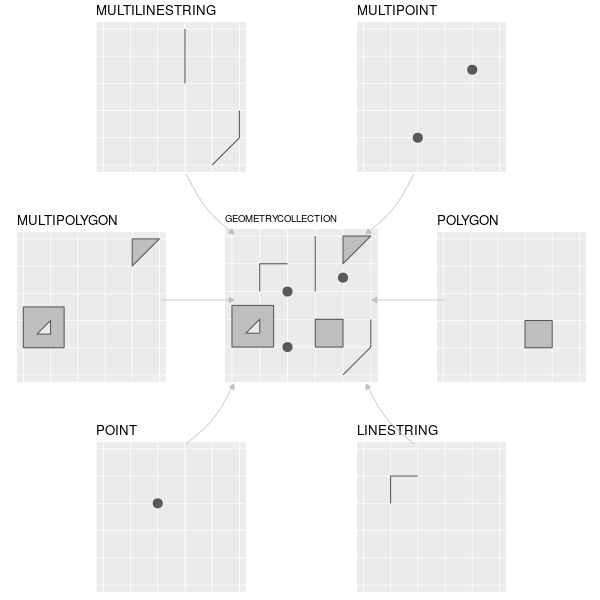
\includegraphics[width=0.6\linewidth]{images/sf-classes} 

}

\caption{Exemple des différents types de géométrie supportés par le package \texttt{sf} (source : \url{https://geocompr.robinlovelace.net/spatial-class.html\#intro-sf})}\label{fig:sfclasses}
\end{figure}

Le package \texttt{sf} est multitâche, il permet de : lire et écrire des fichiers de
données spatiales via la bibliothèque
\href{https://www.osgeo.org/projects/geos/}{GEOS} ; faire des opérations géométriques
via la bibliothèque \href{https://gdal.org/}{GDAL} ; mais aussi représenter et
transformer des systèmes de coordonnées projetées, à partir de la
bibliothèque \href{https://proj.org/}{PROJ}.

\hypertarget{lecture-des-fichiers-de-donnuxe9es-spatiales-pour-les-vecteurs}{%
\subsubsection{Lecture des fichiers de données spatiales pour les vecteurs}\label{lecture-des-fichiers-de-donnuxe9es-spatiales-pour-les-vecteurs}}

Pour avoir un aperçu des objets \texttt{sf} sous R, nous allons prendre pour exemple
les données de localisation des Réserves Naturelles Nationales (RNN) de la
France métropolitaine (Tableau \ref{tab:data-rnn}). Ces données proviennent de
l'Inventaire National du Patrimoine Naturel
(\href{https://inpn.mnhn.fr/accueil/index}{INPN}) et elles sont trouvables sur le
\href{https://www.data.gouv.fr/fr/datasets/inpn-donnees-du-programme-espaces-proteges/}{site du gouvernement}.

Plusieurs formats de fichier peuvent être utilisés pour stocker les données des
vecteurs. Les plus utilisés sont le format \emph{Shapefile} (\textbf{.shp}) de la société
ESRI, les formats \emph{Keyhole Markup Language} (\textbf{.kml}) de Google (et qui peut
être compressé sous le format \textbf{.kmz}), ou aussi le format \emph{Geographic Markup
Language} (\textbf{.gml}) développé par l'OGC.

Concernant les données spatiales des RNN, elles sont téléchargeables au format
\emph{Shapefile}. Il faut alors savoir que le format \emph{Shapefile} est toujours
accompagné d'autres fichiers, dont les plus importants sont le fichier \textbf{.dbf}
contenant les données attributaires, ainsi que le fichier \textbf{.shx} contenant
l'index de la géométrie. Le fichier \textbf{.shp} contient, lui, les caractéristiques
géométriques des différentes entités. C'est pour cela que lorsqu'on télécharge
des données au format \emph{Shapefile}, on télécharge en réalité tout un dossier
contenant plusieurs fichiers.



Une fois le package \texttt{sf} chargé, pour lire les données spatiales il faut
utiliser la fonction \texttt{st\_read()}. Pour cet exemple, il suffit alors de lui
donner le chemin d'accès au fichier \textbf{.shp}. Les autres fichiers qui lui sont
liés doivent être stockés au même endroit. Pour plus d'informations sur les
différents paramètres et les différentes possibilités de cette fonction, il ne
faut pas hésiter à aller lire sa documentation.

\begin{Shaded}
\begin{Highlighting}[]
\KeywordTok{library}\NormalTok{(}\StringTok{"sf"}\NormalTok{) }\CommentTok{\# Chargement du package sf}

\CommentTok{\# Lecture de la base de données}
\NormalTok{data\_rnn \textless{}{-}}\StringTok{ }\KeywordTok{st\_read}\NormalTok{(}\StringTok{"examples/rnn2019\_12/N\_ENP\_RNN\_S\_000.shp"}\NormalTok{)}
\end{Highlighting}
\end{Shaded}

\begin{verbatim}
## Reading layer `N_ENP_RNN_S_000' from data source `/home/alexis/Documents/doc Alexis Merot/Mon_aide_memoire/examples/rnn2019_12/N_ENP_RNN_S_000.shp' using driver `ESRI Shapefile'
## Simple feature collection with 151 features and 30 fields
## geometry type:  MULTIPOLYGON
## dimension:      XY
## bbox:           xmin: 107791.7 ymin: 6145089 xmax: 1077646 ymax: 7109090
## projected CRS:  RGF93 / Lambert-93
\end{verbatim}

Des informations intéressantes sont alors affichées après lecture du fichier. On peut y lire dans l'ordre : le chemin d'accès du fichier source ; le type de l'objet ainsi créé avec quelques informations sur ses éléments,

En regardant l'objet \texttt{sf} alors créé, on peut s'apercevoir qu'il a la forme d'un
tableau de données comme on a l'habitude de voir. Cette caractéristique permet
de le manipuler facilement, notamment via le package
\href{http://larmarange.github.io/analyse-R/manipuler-les-donnees-avec-dplyr.html}{\texttt{dplyr}}.

\begin{Shaded}
\begin{Highlighting}[]
\CommentTok{\# Visualisation du tableau de données}
\NormalTok{knitr}\OperatorTok{::}\KeywordTok{kable}\NormalTok{(data\_rnn, }\DataTypeTok{caption =} \StringTok{"(ref:data{-}rnn)"}\NormalTok{) }\OperatorTok{\%\textgreater{}\%}
\StringTok{  }\NormalTok{kableExtra}\OperatorTok{::}\KeywordTok{kable\_styling}\NormalTok{(}
    \DataTypeTok{bootstrap\_options =} \KeywordTok{c}\NormalTok{(}\StringTok{"striped"}\NormalTok{, }\StringTok{"hovered"}\NormalTok{, }\StringTok{"condensed"}\NormalTok{, }\StringTok{"responsive"}\NormalTok{),}
    \DataTypeTok{font\_size =} \DecValTok{12}\NormalTok{,}
    \DataTypeTok{fixed\_thead =} \OtherTok{TRUE}
\NormalTok{  ) }\OperatorTok{\%\textgreater{}\%}
\StringTok{  }\NormalTok{kableExtra}\OperatorTok{::}\KeywordTok{scroll\_box}\NormalTok{(}\DataTypeTok{width =} \StringTok{"100\%"}\NormalTok{, }\DataTypeTok{height =} \StringTok{"400px"}\NormalTok{)}
\end{Highlighting}
\end{Shaded}

\label{tab:data-rnn}Jeu de données spatiales montrant les Réserves Naturelles Nationales de la France métropolitaine.

ID\_LOCAL

PRN\_ASSO

CODE\_R\_ENP

NOM\_SITE

DATE\_CREA

MODIF\_ADM

MODIF\_GEO

URL\_FICHE

SURF\_OFF

ACTE\_DEB

ACTE\_FIN

GEST\_SITE

OPERATEUR

SRC\_GEOM

SRC\_ANNEE

MARIN

P1\_NATURE

P2\_CULTURE

P3\_PAYSAGE

P4\_GEOLOGI

P5\_SPELEO

P6\_ARCHEO

P7\_PALEOB

P8\_ANTHROP

P9\_SCIENCE

P10\_PUBLIC

P11\_DD

P12\_AUTRE

ID\_MNHN

PRECISION

geometry

RNN70

NA

RNN

Mas Larrieu

1984-07-17

NA

2011-10-19

\url{https://inpn.mnhn.fr/espace/protege/FR3600070}

145.0470

FR360006719840722

NA

NA

DREAL LANGUEDOC-ROUSSILLON

BDP /TCHV2

2010

F

N

N

N

N

N

N

N

N

N

N

N

N

FR3600070

M

MULTIPOLYGON (((703769 6164\ldots{}

RNN71

NA

RNN

Py

1984-09-17

NA

2011-10-19

\url{https://inpn.mnhn.fr/espace/protege/FR3600071}

3929.9460

FR360007119840919

NA

NA

DREAL LANGUEDOC-ROUSSILLON

BDP

2010

F

N

N

N

N

N

N

N

N

N

N

N

N

FR3600071

M

MULTIPOLYGON (((648289.9 61\ldots{}

RNN72

NA

RNN

Mantet

1984-09-17

NA

2011-10-19

\url{https://inpn.mnhn.fr/espace/protege/FR3600072}

3028.3470

FR360007119840919

NA

NA

DREAL LANGUEDOC-ROUSSILLON

BDP

2010

F

N

N

N

N

N

N

N

N

N

N

N

N

FR3600072

M

MULTIPOLYGON (((641189.8 61\ldots{}

RNN73

NA

RNN

Région De Digne

1984-10-31

NA

NA

\url{https://inpn.mnhn.fr/espace/protege/FR3600073}

269.3161

FR360007319841106

NA

NA

DREAL PROVENCE-ALPES-COTE-D'AZUR

NA

NA

F

N

N

N

N

N

N

N

N

N

N

N

N

FR3600073

NA

MULTIPOLYGON (((966430.2 63\ldots{}

RNN74

NA

RNN

Hauts Plateaux Du Vercors

1985-02-27

NA

NA

\url{https://inpn.mnhn.fr/espace/protege/FR3600074}

16661.8300

FR360007419850228

NA

NA

DREAL RHONE-ALPES

NA

NA

F

N

N

N

N

N

N

N

N

N

N

N

N

FR3600074

NA

MULTIPOLYGON (((899491.5 64\ldots{}

RNN76

NA

RNN

Étang De La Mazière

1985-06-19

NA

NA

\url{https://inpn.mnhn.fr/espace/protege/FR3600076}

68.3648

FR360007619850622

NA

NA

DREAL AQUITAINE

NA

NA

F

N

N

N

N

N

N

N

N

N

N

N

N

FR3600076

NA

MULTIPOLYGON (((483422 6368\ldots{}

RNN42

NA

RNN

Domaine De Beauguillot

1980-01-17

NA

NA

\url{https://inpn.mnhn.fr/espace/protege/FR3600042}

685.9300

FR360004219800122

NA

NA

DREAL BASSE-NORMANDIE

NA

NA

T

N

N

N

N

N

N

N

N

N

N

N

N

FR3600042

NA

MULTIPOLYGON (((397279.2 69\ldots{}

RNN43

NA

RNN

Delta De La Dranse

1980-01-17

1994-02-08

NA

\url{https://inpn.mnhn.fr/espace/protege/FR3600043}

52.0000

FR360004219800122

FR360004319940212

NA

DREAL RHONE-ALPES

NA

NA

F

N

N

N

N

N

N

N

N

N

N

N

N

FR3600043

NA

MULTIPOLYGON (((969867.1 65\ldots{}

RNN48

NA

RNN

Lac De Grand-Lieu

1980-09-10

NA

NA

\url{https://inpn.mnhn.fr/espace/protege/FR3600048}

2694.6030

FR360004719800912

NA

NA

DREAL PAYS-DE-LA-LOIRE

NA

NA

F

N

N

N

N

N

N

N

N

N

N

N

N

FR3600048

NA

MULTIPOLYGON (((345409.5 66\ldots{}

RNN50

NA

RNN

Passy

1980-12-22

NA

NA

\url{https://inpn.mnhn.fr/espace/protege/FR3600050}

2000.0000

FR360005019801223

NA

NA

DREAL RHONE-ALPES

NA

NA

F

N

N

N

N

N

N

N

N

N

N

N

N

FR3600050

NA

MULTIPOLYGON (((998218 6552\ldots{}

RNN55

NA

RNN

Coteau De Mesnil Soleil

1981-08-28

NA

NA

\url{https://inpn.mnhn.fr/espace/protege/FR3600055}

25.0000

FR360005419810915

NA

NA

DREAL BASSE-NORMANDIE

NA

NA

F

N

N

N

N

N

N

N

N

N

N

N

N

FR3600055

NA

MULTIPOLYGON (((469046.4 68\ldots{}

RNN58

NA

RNN

Marais D'Isle

1981-10-05

NA

NA

\url{https://inpn.mnhn.fr/espace/protege/FR3600058}

47.5245

FR360005819811008

NA

NA

DREAL PICARDIE

NA

NA

F

N

N

N

N

N

N

N

N

N

N

N

N

FR3600058

NA

MULTIPOLYGON (((721857.1 69\ldots{}

RNN60

NA

RNN

Petite Camargue Alsacienne

1982-06-11

2006-07-27

NA

\url{https://inpn.mnhn.fr/espace/protege/FR3600060}

904.0000

FR360006019820616

FR360006020060728

NA

DREAL ALSACE

NA

NA

F

N

N

N

N

N

N

N

N

N

N

N

N

FR3600060

NA

MULTIPOLYGON (((1041131 673\ldots{}

RNN100

NA

RNN

Plan De Tueda

1990-07-12

NA

NA

\url{https://inpn.mnhn.fr/espace/protege/FR3600100}

1112.7050

FR360010019900719

NA

NA

DREAL RHONE-ALPES

NA

NA

F

N

N

N

N

N

N

N

N

N

N

N

N

FR3600100

NA

MULTIPOLYGON (((980502.3 64\ldots{}

RNN101

NA

RNN

Hauts De Villaroger

1991-01-28

NA

NA

\url{https://inpn.mnhn.fr/espace/protege/FR3600101}

1114.6800

FR360010119910202

NA

NA

DREAL RHONE-ALPES

NA

NA

F

N

N

N

N

N

N

N

N

N

N

N

N

FR3600101

NA

MULTIPOLYGON (((1001112 650\ldots{}

RNN102

NA

RNN

Sangsurière Et De L'Adriennerie

1991-02-26

NA

NA

\url{https://inpn.mnhn.fr/espace/protege/FR3600102}

396.0695

FR360010219910302

NA

NA

DREAL BASSE-NORMANDIE

NA

NA

F

N

N

N

N

N

N

N

N

N

N

N

N

FR3600102

NA

MULTIPOLYGON (((367811.2 69\ldots{}

RNN103

NA

RNN

Carlaveyron

1991-03-05

NA

NA

\url{https://inpn.mnhn.fr/espace/protege/FR3600103}

598.9005

FR360010319910309

NA

NA

DREAL RHONE-ALPES

NA

NA

F

N

N

N

N

N

N

N

N

N

N

N

N

FR3600103

NA

MULTIPOLYGON (((995638.4 65\ldots{}

RNN104

NA

RNN

Vireux-Molhain

1991-03-14

NA

NA

\url{https://inpn.mnhn.fr/espace/protege/FR3600104}

1.8200

FR360010419910320

NA

NA

DREAL CHAMPAGNE-ARDENNE

NA

NA

F

N

N

N

N

N

N

N

N

N

N

N

N

FR3600104

NA

MULTIPOLYGON (((822291.7 70\ldots{}

RNN106

NA

RNN

Ile De Rhinau

1991-09-06

NA

NA

\url{https://inpn.mnhn.fr/espace/protege/FR3600106}

306.7179

FR360010619910913

NA

NA

DREAL ALSACE

NA

NA

F

N

N

N

N

N

N

N

N

N

N

N

N

FR3600106

NA

MULTIPOLYGON (((1045884 680\ldots{}

RNN107

NA

RNN

Vallon De Bérard

1992-09-17

NA

NA

\url{https://inpn.mnhn.fr/espace/protege/FR3600107}

539.6997

FR360010719920923

NA

NA

DREAL RHONE-ALPES

NA

NA

F

N

N

N

N

N

N

N

N

N

N

N

N

FR3600107

NA

MULTIPOLYGON (((998218 6552\ldots{}

RNN108

NA

RNN

Iroise

1992-10-12

NA

NA

\url{https://inpn.mnhn.fr/espace/protege/FR3600108}

39.4258

FR360010819921020

NA

NA

DREAL BRETAGNE

NA

NA

F

N

N

N

N

N

N

N

N

N

N

N

N

FR3600108

NA

MULTIPOLYGON (((110439.8 68\ldots{}

RNN111

NA

RNN

Venec

1993-02-09

NA

NA

\url{https://inpn.mnhn.fr/espace/protege/FR3600111}

47.7800

FR360011119930216

NA

NA

DREAL BRETAGNE

NA

NA

F

N

N

N

N

N

N

N

N

N

N

N

N

FR3600111

NA

MULTIPOLYGON (((190742.2 68\ldots{}

RNN113

NA

RNN

Vallée D'Eyne

1993-03-18

NA

2011-10-19

\url{https://inpn.mnhn.fr/espace/protege/FR3600113}

1177.3060

FR360011319930325

NA

NA

DREAL LANGUEDOC-ROUSSILLON

BDP

2008

F

N

N

N

N

N

N

N

N

N

N

N

N

FR3600113

M

MULTIPOLYGON (((625131.6 61\ldots{}

RNN117

NA

RNN

Sainte-Victoire

1994-03-01

NA

NA

\url{https://inpn.mnhn.fr/espace/protege/FR3600117}

139.8431

FR360011719940303

NA

NA

DREAL PROVENCE-ALPES-COTE-D'AZUR

NA

NA

F

N

N

N

N

N

N

N

N

N

N

N

N

FR3600117

NA

MULTIPOLYGON (((906425 6273\ldots{}

RNN118

NA

RNN

Baie De Somme

1994-03-21

NA

NA

\url{https://inpn.mnhn.fr/espace/protege/FR3600118}

0.0000

FR360011819940323

NA

NA

DREAL PICARDIE

NA

NA

T

N

N

N

N

N

N

N

N

N

N

N

N

FR3600118

NA

MULTIPOLYGON (((594333.7 70\ldots{}

RNN119

NA

RNN

Val D'Allier

1994-03-25

NA

NA

\url{https://inpn.mnhn.fr/espace/protege/FR3600119}

1450.0000

FR360011919940329

NA

NA

DREAL AUVERGNE

NA

NA

F

N

N

N

N

N

N

N

N

N

N

N

N

FR3600119

NA

MULTIPOLYGON (((724921.3 66\ldots{}

RNN121

NA

RNN

Marais De Müllembourg

1994-08-30

NA

NA

\url{https://inpn.mnhn.fr/espace/protege/FR3600121}

48.3900

FR360012119940901

NA

NA

DREAL PAYS-DE-LA-LOIRE

NA

NA

F

N

N

N

N

N

N

N

N

N

N

N

N

FR3600121

NA

MULTIPOLYGON (((302498.6 66\ldots{}

RNN30

NA

RNN

Mare De Vauville

1976-05-06

2002-02-27

NA

\url{https://inpn.mnhn.fr/espace/protege/FR3600030}

60.2596

FR360003019760610

FR360003020020306

NA

DREAL BASSE-NORMANDIE

NA

NA

F

N

N

N

N

N

N

N

N

N

N

N

N

FR3600030

NA

MULTIPOLYGON (((349724.6 69\ldots{}

RNN32

NA

RNN

Sept-Iles

1976-10-18

NA

NA

\url{https://inpn.mnhn.fr/espace/protege/FR3600032}

280.0000

FR360003219761030

NA

NA

DREAL BRETAGNE

NA

NA

T

N

N

N

N

N

N

N

N

N

N

N

N

FR3600032

NA

MULTIPOLYGON (((223603.9 68\ldots{}

RNN33

NA

RNN

Marais Communal De Saint-Denis-Du-Payré

1976-10-18

2002-05-03

NA

\url{https://inpn.mnhn.fr/espace/protege/FR3600033}

206.4385

FR360003219761030

FR360003320020505

NA

DREAL PAYS-DE-LA-LOIRE

NA

NA

F

N

N

N

N

N

N

N

N

N

N

N

N

FR3600033

NA

MULTIPOLYGON (((374127.2 65\ldots{}

RNN36

NA

RNN

Roc De Chère

1977-11-02

NA

NA

\url{https://inpn.mnhn.fr/espace/protege/FR3600036}

68.0000

FR360003519771110

NA

NA

DREAL RHONE-ALPES

NA

NA

F

N

N

N

N

N

N

N

N

N

N

N

N

FR3600036

NA

MULTIPOLYGON (((948141.8 65\ldots{}

RNN37

NA

RNN

Vallées De La Grand-Pierre Et De Vitain

1979-08-23

1982-03-26

NA

\url{https://inpn.mnhn.fr/espace/protege/FR3600037}

296.0000

FR360003719790828

FR360003719820401

NA

DREAL CENTRE

NA

NA

F

N

N

N

N

N

N

N

N

N

N

N

N

FR3600037

NA

MULTIPOLYGON (((572306.9 67\ldots{}

RNN38

NA

RNN

Contamines-Montjoie

1979-08-29

NA

NA

\url{https://inpn.mnhn.fr/espace/protege/FR3600038}

0.0000

FR360003819790907

NA

NA

DREAL RHONE-ALPES

NA

NA

F

N

N

N

N

N

N

N

N

N

N

N

N

FR3600038

NA

MULTIPOLYGON (((990290.2 65\ldots{}

RNN40

NA

RNN

Étang Saint-Ladre

1979-09-11

1988-02-05

NA

\url{https://inpn.mnhn.fr/espace/protege/FR3600040}

13.3699

FR360004019790921

FR360004019880211

NA

DREAL PICARDIE

NA

NA

F

N

N

N

N

N

N

N

N

N

N

N

N

FR3600040

NA

MULTIPOLYGON (((655398.4 69\ldots{}

RNN12

NA

RNN

Haute Vallée Du Torrent De Saint-Pierre

1974-05-15

NA

NA

\url{https://inpn.mnhn.fr/espace/protege/FR3600012}

20.0000

FR360001119740525

NA

NA

DREAL PROVENCE-ALPES-COTE-D'AZUR

NA

NA

F

N

N

N

N

N

N

N

N

N

N

N

N

FR3600012

NA

MULTIPOLYGON (((971095.6 64\ldots{}

RNN15

NA

RNN

Cirque Du Grand Lac Des Estaris

1974-05-15

NA

NA

\url{https://inpn.mnhn.fr/espace/protege/FR3600015}

145.0000

FR360001119740525

NA

NA

DREAL PROVENCE-ALPES-COTE-D'AZUR

NA

NA

F

N

N

N

N

N

N

N

N

N

N

N

N

FR3600015

NA

MULTIPOLYGON (((964968 6409\ldots{}

RNN16

NA

RNN

Versant Nord Des Pics Du Combeynot

1974-05-15

NA

NA

\url{https://inpn.mnhn.fr/espace/protege/FR3600016}

685.0000

FR360001119740525

NA

NA

DREAL PROVENCE-ALPES-COTE-D'AZUR

NA

NA

F

N

N

N

N

N

N

N

N

N

N

N

N

FR3600016

NA

MULTIPOLYGON (((969975.9 64\ldots{}

RNN18

NA

RNN

Aiguilles Rouges

1974-08-23

2010-01-27

NA

\url{https://inpn.mnhn.fr/espace/protege/FR3600018}

3276.0000

FR360001819740904

FR360001820100129

NA

DREAL RHONE-ALPES

NA

NA

F

N

N

N

N

N

N

N

N

N

N

N

N

FR3600018

NA

MULTIPOLYGON (((996497.9 65\ldots{}

RNN22

NA

RNN

Camargue

1975-04-24

1984-09-12

NA

\url{https://inpn.mnhn.fr/espace/protege/FR3600022}

13117.5000

FR360002219750510

FR360002219850214

NA

DREAL PROVENCE-ALPES-COTE-D'AZUR

NA

NA

F

N

N

N

N

N

N

N

N

N

N

N

N

FR3600022

NA

MULTIPOLYGON (((824949.2 62\ldots{}

RNN25

NA

RNN

Roque-Haute

1975-12-09

1998-07-23

2011-10-19

\url{https://inpn.mnhn.fr/espace/protege/FR3600025}

154.6390

FR360002519751211

FR360002519980729

NA

DREAL LANGUEDOC-ROUSSILLON

BDP

2008

F

N

N

N

N

N

N

N

N

N

N

N

N

FR3600025

M

MULTIPOLYGON (((730266 6245\ldots{}

RNN27

NA

RNN

L'Estagnol

1975-11-19

NA

2011-10-19

\url{https://inpn.mnhn.fr/espace/protege/FR3600027}

78.3660

FR360002619751218

NA

NA

DREAL LANGUEDOC-ROUSSILLON

BDP

2008

F

N

N

N

N

N

N

N

N

N

N

N

N

FR3600027

M

MULTIPOLYGON (((767930.2 62\ldots{}

RNN28

NA

RNN

Forêt Domaniale De Cerisy

1976-03-02

NA

NA

\url{https://inpn.mnhn.fr/espace/protege/FR3600028}

2124.0000

FR360002819760330

NA

NA

DREAL BASSE-NORMANDIE

NA

NA

F

N

N

N

N

N

N

N

N

N

N

N

N

FR3600028

NA

MULTIPOLYGON (((418987.2 69\ldots{}

RNN1

NA

RNN

Lac Luitel

1961-03-15

1991-04-03

NA

\url{https://inpn.mnhn.fr/espace/protege/FR3600001}

17.1580

FR360000119610315

FR360000119910409

NA

DREAL RHONE-ALPES

NA

NA

F

N

N

N

N

N

N

N

N

N

N

N

N

FR3600001

NA

MULTIPOLYGON (((924113.6 64\ldots{}

RNN2

NA

RNN

Tignes-Champagny

1963-07-24

1973-08-10

NA

\url{https://inpn.mnhn.fr/espace/protege/FR3600002}

999.0000

FR360000219640312

FR360000219730913

NA

DREAL RHONE-ALPES

NA

NA

F

N

N

N

N

N

N

N

N

N

N

N

N

FR3600002

NA

MULTIPOLYGON (((1002246 649\ldots{}

RNN4

NA

RNN

Néouvielle

1968-05-08

1994-03-04

NA

\url{https://inpn.mnhn.fr/espace/protege/FR3600004}

2313.0000

FR360000419940306

FR360000419940306

NA

DREAL MIDI-PYRENEES

BDP

2013

F

N

N

N

N

N

N

N

N

N

N

N

N

FR3600004

M

MULTIPOLYGON (((468349.1 62\ldots{}

RNN6

NA

RNN

Forêt De La Massane

1973-07-30

1991-03-29

2011-10-19

\url{https://inpn.mnhn.fr/espace/protege/FR3600006}

335.9860

FR360000619730812

FR360000619910517

NA

DREAL LANGUEDOC-ROUSSILLON

BDP

2010

F

N

N

N

N

N

N

N

N

N

N

N

N

FR3600006

M

MULTIPOLYGON (((702268 6155\ldots{}

RNN7

NA

RNN

Grande Sassière

1973-08-10

NA

NA

\url{https://inpn.mnhn.fr/espace/protege/FR3600007}

2230.0000

FR360000219730913

NA

NA

DREAL RHONE-ALPES

NA

NA

F

N

N

N

N

N

N

N

N

N

N

N

N

FR3600007

NA

MULTIPOLYGON (((1016009 649\ldots{}

RNN8

NA

RNN

Tourbière De Mathon

1973-09-26

NA

NA

\url{https://inpn.mnhn.fr/espace/protege/FR3600008}

16.0000

FR360000819731026

NA

NA

DREAL BASSE-NORMANDIE

NA

NA

F

N

N

N

N

N

N

N

N

N

N

N

N

FR3600008

NA

MULTIPOLYGON (((370785.1 69\ldots{}

RNN9

NA

RNN

Cerbère - Banyuls

1990-09-06

NA

2011-10-19

\url{https://inpn.mnhn.fr/espace/protege/FR3600009}

650.0000

FR360000919740305

FR360000919900906

NA

DREAL LANGUEDOC-ROUSSILLON

BDP

2010

T

N

N

N

N

N

N

N

N

N

N

N

N

FR3600009

M

MULTIPOLYGON (((713598.4 61\ldots{}

RNN10

NA

RNN

Saint-Nicolas-Des-Glénan

1974-04-18

NA

NA

\url{https://inpn.mnhn.fr/espace/protege/FR3600010}

1.5255

FR360001019740502

NA

NA

DREAL BRETAGNE

NA

NA

F

N

N

N

N

N

N

N

N

N

N

N

N

FR3600010

NA

MULTIPOLYGON (((175976.1 67\ldots{}

RNN11

NA

RNN

Haute Vallée De La Rivière De La Séveraisse

1974-05-15

NA

NA

\url{https://inpn.mnhn.fr/espace/protege/FR3600011}

155.0000

FR360001119740525

NA

NA

DREAL PROVENCE-ALPES-COTE-D'AZUR

NA

NA

F

N

N

N

N

N

N

N

N

N

N

N

N

FR3600011

NA

MULTIPOLYGON (((958718 6419\ldots{}

RNN63

NA

RNN

François Le Bail (Ile De Groix)

1982-12-23

NA

NA

\url{https://inpn.mnhn.fr/espace/protege/FR3600063}

42.8187

FR360006319830114

NA

NA

DREAL BRETAGNE

NA

NA

T

N

N

N

N

N

N

N

N

N

N

N

N

FR3600063

NA

MULTIPOLYGON (((217175.7 67\ldots{}

RNN65

NA

RNN

Prés Salés D'Arès Et De Lège-Cap-Ferret

1983-09-07

NA

NA

\url{https://inpn.mnhn.fr/espace/protege/FR3600065}

495.0000

FR360006519830913

NA

NA

DREAL AQUITAINE

NA

NA

T

N

N

N

N

N

N

N

N

N

N

N

N

FR3600065

NA

MULTIPOLYGON (((371156.1 64\ldots{}

RNN67

NA

RNN

Bagnas

1983-11-22

1984-07-17

2011-10-19

\url{https://inpn.mnhn.fr/espace/protege/FR3600067}

561.2889

FR360006719831124

FR360006719840722

NA

DREAL LANGUEDOC-ROUSSILLON

BDP

2008

T

N

N

N

N

N

N

N

N

N

N

N

N

FR3600067

M

MULTIPOLYGON (((742230.4 62\ldots{}

RNN68

NA

RNN

Marais De Lavours

1984-03-22

NA

NA

\url{https://inpn.mnhn.fr/espace/protege/FR3600068}

473.3892

FR360006819840324

NA

NA

DREAL RHONE-ALPES

NA

NA

F

N

N

N

N

N

N

N

N

N

N

N

N

FR3600068

NA

MULTIPOLYGON (((913546.6 65\ldots{}

PCRNN86001

NA

RNN

Pinail

1980-01-30

1980-10-23

NA

\url{https://inpn.mnhn.fr/espace/protege/FR3600044}

135.0000

FR360004419800216

FR360004419801031

GEREPI

DREAL Poitou-Charentes

NA

NA

F

T

F

F

F

F

F

F

F

F

F

F

F

FR3600044

NA

MULTIPOLYGON (((510443.3 66\ldots{}

PCRNN17002

NA

RNN

Marais D'Yves

1981-08-28

NA

NA

\url{https://inpn.mnhn.fr/espace/protege/FR3600053}

192.4089

FR360005419810915

NA

LPO

DREAL Poitoui-Charentes

NA

NA

F

T

F

F

F

F

F

F

F

F

F

F

F

FR3600053

NA

MULTIPOLYGON (((387065.3 65\ldots{}

PCRNN79001

NA

RNN

Toarcien

1987-11-23

NA

NA

\url{https://inpn.mnhn.fr/espace/protege/FR3600091}

0.6100

FR360009119871127

NA

Communauté de Communes du Thouarsais

DREAL Poitou-Charentes

NA

NA

F

T

F

F

T

F

F

F

F

T

F

F

F

FR3600091

NA

MULTIPOLYGON (((453539.9 66\ldots{}

RNN114

NA

RNN

Chalmessin

1993-09-02

NA

NA

\url{https://inpn.mnhn.fr/espace/protege/FR3600114}

123.6502

FR360011419930908

NA

NA

DREAL CHAMPAGNE-ARDENNE

NA

NA

F

N

N

N

N

N

N

N

N

N

N

N

N

FR3600114

NA

MULTIPOLYGON (((856949.5 67\ldots{}

RNN126

NA

RNN

Frankenthal-Missheimle

1995-10-19

NA

NA

\url{https://inpn.mnhn.fr/espace/protege/FR3600126}

746.3627

FR360012619951020

NA

NA

DREAL ALSACE

NA

NA

F

N

N

N

N

N

N

N

N

N

N

N

N

FR3600126

NA

MULTIPOLYGON (((1001643 678\ldots{}

RNN130

NA

RNN

Baie De L'Aiguillon (Vendée)

1996-07-09

NA

NA

\url{https://inpn.mnhn.fr/espace/protege/FR3600130}

2300.0000

FR360013019960710

NA

NA

DREAL PAYS-DE-LA-LOIRE

NA

NA

T

N

N

N

N

N

N

N

N

N

N

N

N

FR3600130

NA

MULTIPOLYGON (((379817.4 65\ldots{}

RNN79

NA

RNN

Ile De La Platière

1986-03-06

NA

NA

\url{https://inpn.mnhn.fr/espace/protege/FR3600079}

485.0000

FR360007919860311

NA

NA

DREAL RHONE-ALPES

NA

NA

F

N

N

N

N

N

N

N

N

N

N

N

N

FR3600079

NA

MULTIPOLYGON (((839181.9 64\ldots{}

RNN80

NA

RNN

Saint-Quentin-En-Yvelines

1986-03-14

1987-04-27

NA

\url{https://inpn.mnhn.fr/espace/protege/FR3600080}

0.0000

FR360008019860320

FR360008019870502

NA

DRIEE ILE-DE-FRANCE

NA

NA

F

N

N

N

N

N

N

N

N

N

N

N

N

FR3600080

NA

MULTIPOLYGON (((626433.2 68\ldots{}

RNN81

NA

RNN

Prats-De-Mollo-La-Preste

1986-03-14

NA

2011-10-19

\url{https://inpn.mnhn.fr/espace/protege/FR3600081}

2185.9070

FR360008019860320

NA

NA

DREAL LANGUEDOC-ROUSSILLON

BDP

2010

F

N

N

N

N

N

N

N

N

N

N

N

N

FR3600081

M

MULTIPOLYGON (((653725.1 61\ldots{}

RNN82

NA

RNN

Conat

1986-10-23

NA

2011-10-19

\url{https://inpn.mnhn.fr/espace/protege/FR3600082}

548.8030

FR360008219861029

NA

NA

DREAL LANGUEDOC-ROUSSILLON

BDP

2010

F

N

N

N

N

N

N

N

N

N

N

N

N

FR3600082

M

MULTIPOLYGON (((642968.8 61\ldots{}

RNN83

NA

RNN

Jujols

1986-10-23

NA

2011-10-19

\url{https://inpn.mnhn.fr/espace/protege/FR3600083}

472.3572

FR360008219861029

NA

NA

DREAL LANGUEDOC-ROUSSILLON

BDP

2010

F

N

N

N

N

N

N

N

N

N

N

N

N

FR3600083

M

MULTIPOLYGON (((641782.3 61\ldots{}

RNN84

NA

RNN

Nohèdes

1986-10-23

NA

2011-10-19

\url{https://inpn.mnhn.fr/espace/protege/FR3600084}

2137.2330

FR360008219861029

NA

NA

DREAL LANGUEDOC-ROUSSILLON

BDP

2010

F

N

N

N

N

N

N

N

N

N

N

N

N

FR3600084

M

MULTIPOLYGON (((642958.1 61\ldots{}

RNN88

NA

RNN

Grotte du TM71

1987-08-17

NA

2011-10-19

\url{https://inpn.mnhn.fr/espace/protege/FR3600088}

96.0275

FR360008819870821

NA

NA

DREAL LANGUEDOC-ROUSSILLON

BDP

2008

F

N

N

N

N

N

N

N

N

N

N

N

N

FR3600088

M

MULTIPOLYGON (((626237.1 61\ldots{}

RNN90

NA

RNN

Lubéron

1987-09-16

NA

NA

\url{https://inpn.mnhn.fr/espace/protege/FR3600090}

312.1654

FR360009019871010

NA

NA

DREAL PROVENCE-ALPES-COTE-D'AZUR

NA

NA

F

N

N

N

N

N

N

N

N

N

N

N

N

FR3600090

NA

MULTIPOLYGON (((873599.8 62\ldots{}

RNN96

FR9500096

RNN

Sites Géologiques Du Département De L'Essonne

1989-07-17

2011-04-20

NA

\url{https://inpn.mnhn.fr/espace/protege/FR3600096}

27.0000

FR360009619890719

FR360009620110422

NA

DRIEE ILE-DE-FRANCE

NA

NA

F

N

N

N

N

N

N

N

N

N

N

N

N

FR3600096

NA

MULTIPOLYGON (((640946.9 68\ldots{}

RNN97

NA

RNN

Forêt D'Offendorf

1989-07-28

NA

NA

\url{https://inpn.mnhn.fr/espace/protege/FR3600097}

59.0900

FR360009719890802

NA

NA

DREAL ALSACE

NA

NA

F

N

N

N

N

N

N

N

N

N

N

N

N

FR3600097

NA

MULTIPOLYGON (((1064210 685\ldots{}

RNN98

NA

RNN

Forêt D'Erstein

1989-09-18

NA

NA

\url{https://inpn.mnhn.fr/espace/protege/FR3600098}

179.5525

FR360009819890923

NA

NA

DREAL ALSACE

NA

NA

F

N

N

N

N

N

N

N

N

N

N

N

N

FR3600098

NA

MULTIPOLYGON (((1050862 682\ldots{}

RNN179

NA

RNN

Chaumes Du Verniller

2014-02-13

NA

NA

\url{https://inpn.mnhn.fr/espace/protege/FR3600178}

81.0000

FR360017820140215

NA

NA

DREAL CENTRE

Cadastre

2007

F

T

N

N

N

N

N

N

N

N

N

N

N

FR3600178

M

MULTIPOLYGON (((648108.9 66\ldots{}

RNN26

FR9500026

RNN

Saint-Mesmin

1975-11-19

2006-12-14

NA

\url{https://inpn.mnhn.fr/espace/protege/FR3600026}

263.0000

FR360002619751218

FR360002620061216

NA

DREAL CENTRE

Cadastre

NA

F

N

N

N

N

N

N

N

N

N

N

N

N

FR3600026

M

MULTIPOLYGON (((612753.3 67\ldots{}

RNN78

NA

RNN

Chérine

1985-07-22

2011-09-09

2014-11-19

\url{https://inpn.mnhn.fr/espace/protege/FR3600078}

370.0000

FR360007819850727

FR360007820110911

NA

DREAL CENTRE

Cadastre

2011

F

N

N

N

N

N

N

N

N

N

N

N

N

FR3600078

M

MULTIPOLYGON (((561215.4 66\ldots{}

RNN131

NA

RNN

Marais De Séné

1996-08-21

NA

NA

\url{https://inpn.mnhn.fr/espace/protege/FR3600131}

410.0000

FR360013119960823

NA

NA

DREAL BRETAGNE

NA

NA

F

N

N

N

N

N

N

N

N

N

N

N

N

FR3600131

NA

MULTIPOLYGON (((271525.5 67\ldots{}

RNN133

NA

RNN

Ile Du Rohrschollen

1997-03-04

NA

NA

\url{https://inpn.mnhn.fr/espace/protege/FR3600133}

309.9100

FR360013319970311

NA

NA

DREAL ALSACE

NA

NA

F

N

N

N

N

N

N

N

N

N

N

N

N

FR3600133

NA

MULTIPOLYGON (((1054607 683\ldots{}

RNN134

NA

RNN

Marais De Vesles-Et-Caumont

1997-04-02

NA

NA

\url{https://inpn.mnhn.fr/espace/protege/FR3600134}

108.6726

FR360013419970403

NA

NA

DREAL PICARDIE

NA

NA

F

N

N

N

N

N

N

N

N

N

N

N

N

FR3600134

NA

MULTIPOLYGON (((756210.3 69\ldots{}

RNN135

NA

RNN

Delta De La Sauer

1997-09-02

NA

NA

\url{https://inpn.mnhn.fr/espace/protege/FR3600135}

486.3708

FR360013519970905

NA

NA

DREAL ALSACE

NA

NA

F

N

N

N

N

N

N

N

N

N

N

N

N

FR3600135

NA

MULTIPOLYGON (((1075998 687\ldots{}

RNN136

NA

RNN

Hauts De Chartreuse

1997-10-01

NA

NA

\url{https://inpn.mnhn.fr/espace/protege/FR3600136}

4450.0000

FR360013619971004

NA

NA

DREAL RHONE-ALPES

NA

NA

F

N

N

N

N

N

N

N

N

N

N

N

N

FR3600136

NA

MULTIPOLYGON (((927782.6 64\ldots{}

RNN137

NA

RNN

Estuaire De La Seine

1997-12-30

2004-11-09

NA

\url{https://inpn.mnhn.fr/espace/protege/FR3600137}

8528.0000

FR360013719980101

FR360013720041110

NA

DREAL HAUTE-NORMANDIE

NA

NA

T

N

N

N

N

N

N

N

N

N

N

N

N

FR3600137

NA

MULTIPOLYGON (((495133.4 69\ldots{}

RNN140

NA

RNN

Baie De Saint-Brieuc

1998-04-28

NA

NA

\url{https://inpn.mnhn.fr/espace/protege/FR3600140}

1140.0000

FR360014019980430

NA

NA

DREAL BRETAGNE

NA

NA

T

N

N

N

N

N

N

N

N

N

N

N

N

FR3600140

NA

MULTIPOLYGON (((281856.9 68\ldots{}

RNN145

NA

RNN

Pointe De Givet

1999-03-04

NA

NA

\url{https://inpn.mnhn.fr/espace/protege/FR3600145}

354.2209

FR360014519990305

NA

NA

DREAL CHAMPAGNE-ARDENNE

NA

NA

F

N

N

N

N

N

N

N

N

N

N

N

N

FR3600145

NA

MULTIPOLYGON (((828592.6 70\ldots{}

PCRNN17005

NA

RNN

Baie De L'Aiguillon (Charente-Maritime)

1999-07-02

1999-07-02

NA

\url{https://inpn.mnhn.fr/espace/protege/FR3600146}

2600.0000

Decret99-557

NA

LPO

DREAL POITOU-CHARENTES

NA

NA

T

N

N

N

N

N

N

N

N

N

N

N

N

FR3600146

NA

MULTIPOLYGON (((383236.1 65\ldots{}

RNN149

NA

RNN

Étang De La Horre

2000-05-09

NA

NA

\url{https://inpn.mnhn.fr/espace/protege/FR3600149}

415.3757

FR360014920000516

NA

NA

DREAL CHAMPAGNE-ARDENNE

NA

NA

F

N

N

N

N

N

N

N

N

N

N

N

N

FR3600149

NA

MULTIPOLYGON (((823087.5 68\ldots{}

RNN150

NA

RNN

La Bailletaz

2000-12-06

NA

NA

\url{https://inpn.mnhn.fr/espace/protege/FR3600150}

495.2332

FR360015020001212

NA

NA

DREAL RHONE-ALPES

NA

NA

F

N

N

N

N

N

N

N

N

N

N

N

N

FR3600150

NA

MULTIPOLYGON (((1016009 649\ldots{}

RNN154

NA

RNN

Forêt D'Orient

2002-07-09

NA

NA

\url{https://inpn.mnhn.fr/espace/protege/FR3600154}

1560.0000

FR360015420020716

NA

NA

DREAL CHAMPAGNE-ARDENNE

NA

NA

F

N

N

N

N

N

N

N

N

N

N

N

N

FR3600154

NA

MULTIPOLYGON (((801050.2 68\ldots{}

RNN155

NA

RNN

La Bassée

2002-10-21

NA

NA

\url{https://inpn.mnhn.fr/espace/protege/FR3600155}

854.6749

FR360015520021024

NA

NA

DRIEE ILE-DE-FRANCE

NA

NA

F

N

N

N

N

N

N

N

N

N

N

N

N

FR3600155

NA

MULTIPOLYGON (((724001.1 68\ldots{}

RNN158

NA

RNN

Étang Des Landes

2004-12-23

NA

NA

\url{https://inpn.mnhn.fr/espace/protege/FR3600158}

165.5842

FR360015820041230

NA

NA

DREAL LIMOUSIN

NA

NA

F

N

N

N

N

N

N

N

N

N

N

N

N

FR3600158

NA

MULTIPOLYGON (((647551.9 65\ldots{}

RNN159

NA

RNN

Pâtis D'Oger Et Du Mesnil-Sur-Oger

2006-06-12

NA

NA

\url{https://inpn.mnhn.fr/espace/protege/FR3600159}

130.6737

FR360015920060614

NA

NA

DREAL CHAMPAGNE-ARDENNE

NA

NA

F

N

N

N

N

N

N

N

N

N

N

N

N

FR3600159

NA

MULTIPOLYGON (((773341.5 68\ldots{}

RNN163

NA

RNN

Ristolas - Mont-Viso

2007-02-08

NA

NA

\url{https://inpn.mnhn.fr/espace/protege/FR3600163}

2295.1771

FR360016320070210

NA

NA

DREAL PROVENCE-ALPES-COTE-D'AZUR

NA

NA

F

N

N

N

N

N

N

N

N

N

N

N

N

FR3600163

NA

MULTIPOLYGON (((1017325 641\ldots{}

62RN3

NA

RNN

Grotte Et Pelouses D'Acquin-Westbécourt Et Coteaux De Wavrans-Sur-L'Aa

2008-03-05

NA

2010-01-26

\url{https://inpn.mnhn.fr/espace/protege/FR3600167}

54.0000

FR360016720080307

NA

NA

DREAL NORD-PAS-DE-CALAIS

NA

NA

F

N

N

N

N

N

N

N

N

N

N

N

N

FR3600167

NA

MULTIPOLYGON (((636276.4 70\ldots{}

5962 RN 1

NA

RNN

Étangs Du Romelaëre

2008-03-05

NA

2010-01-26

\url{https://inpn.mnhn.fr/espace/protege/FR3600168}

104.0000

FR360016720080307

NA

NA

DREAL NORD-PAS-DE-CALAIS

NA

NA

F

N

N

N

N

N

N

N

N

N

N

N

N

FR3600168

NA

MULTIPOLYGON (((649444.9 70\ldots{}

RNN169

NA

RNN

Astroblème De Rochechouart-Chassenon

2008-09-18

NA

NA

\url{https://inpn.mnhn.fr/espace/protege/FR3600169}

50.0000

FR360016920080920

NA

NA

DREAL LIMOUSIN

NA

NA

F

N

N

N

N

N

N

N

N

N

N

N

N

FR3600169

NA

MULTIPOLYGON (((530468.2 65\ldots{}

RNN170

NA

RNN

Coteaux De La Seine

2009-03-30

NA

NA

\url{https://inpn.mnhn.fr/espace/protege/FR3600170}

268.0000

FR360017020090401

NA

NA

DRIEE ILE-DE-FRANCE

NA

NA

F

N

N

N

N

N

N

N

N

N

N

N

N

FR3600170

NA

MULTIPOLYGON (((597720.7 68\ldots{}

RNN171

NA

RNN

Plaine Des Maures

2009-06-23

NA

NA

\url{https://inpn.mnhn.fr/espace/protege/FR3600171}

5276.0000

FR360017120090624

NA

NA

DREAL PROVENCE-ALPES-COTE-D'AZUR

NA

NA

F

N

N

N

N

N

N

N

N

N

N

N

N

FR3600171

NA

MULTIPOLYGON (((981117.5 62\ldots{}

RNN172

NA

RNN

Dunes Et Marais D'Hourtin

2009-12-15

NA

NA

\url{https://inpn.mnhn.fr/espace/protege/FR3600172}

2150.0000

FR360017220091217

NA

NA

DREAL AQUITAINE

NA

NA

F

N

N

N

N

N

N

N

N

N

N

N

N

FR3600172

NA

MULTIPOLYGON (((375990.4 64\ldots{}

RNN174

NA

RNN

Casse De La Belle Henriette

2011-08-31

NA

NA

\url{https://inpn.mnhn.fr/espace/protege/FR3600174}

337.0000

FR360017420110902

NA

NA

DREAL PAYS-DE-LA-LOIRE

NA

NA

T

N

N

N

N

N

N

N

N

N

N

N

N

FR3600174

NA

MULTIPOLYGON (((364447.3 65\ldots{}

RNN175

NA

RNN

Marais Du Vigueirat

2011-11-09

NA

NA

\url{https://inpn.mnhn.fr/espace/protege/FR3600175}

919.0000

FR360017520111115

NA

NA

DREAL PROVENCE-ALPES-COTE-D'AZUR

NA

NA

F

N

N

N

N

N

N

N

N

N

N

N

N

FR3600175

NA

MULTIPOLYGON (((841260.4 62\ldots{}

RNN176

NA

RNN

Massif Forestier De Strasbourg-Neuhof/Illkirch-Graffenstaden

2012-09-10

NA

NA

\url{https://inpn.mnhn.fr/espace/protege/FR3600176}

945.0000

FR360017620120912

NA

NA

DREAL ALSACE

NA

NA

F

N

N

N

N

N

N

N

N

N

N

N

N

FR3600176

NA

MULTIPOLYGON (((1052841 683\ldots{}

RNN177

NA

RNN

Marais Vernier

2013-02-25

NA

NA

\url{https://inpn.mnhn.fr/espace/protege/FR3600177}

148.0000

FR360017720130213

NA

NA

DREAL HAUTE-NORMANDIE

NA

NA

F

N

N

N

N

N

N

N

N

N

N

N

N

FR3600177

NA

MULTIPOLYGON (((518275.1 69\ldots{}

RNN178

FR9500179

RNN

Haut-Rhône Français

2013-12-04

NA

NA

\url{https://inpn.mnhn.fr/espace/protege/FR3600179}

1707.0000

FR360017920131208

NA

NA

DREAL RHONE-ALPES

NA

NA

F

N

N

N

N

N

N

N

N

N

N

N

N

FR3600179

NA

MULTIPOLYGON (((893659.8 65\ldots{}

RNN23

NA

RNN

Sagnes De La Godivelle

1975-06-27

NA

NA

\url{https://inpn.mnhn.fr/espace/protege/FR3600023}

24.0000

FR360002319750712

NA

PNR Volcans d'Auvergne

DREAL AUVERGNE

Cadastre

2012

F

T

N

N

N

N

N

N

N

N

N

N

N

FR3600023

M

MULTIPOLYGON (((694417.9 64\ldots{}

RNN180

NA

RNN

Géologique du Lot

2015-06-02

NA

NA

\url{https://inpn.mnhn.fr/espace/protege/FR3600180}

800.0000

FR360018020150602

NA

NA

DREAL MIDI-PYRENEES

BDP

2014

F

N

N

N

N

N

N

N

N

O

N

N

O

FR3600180

M

MULTIPOLYGON (((595981.5 63\ldots{}

PCRNN17003

NA

RNN

Réserve Naturelle De Moëze-Oléron

1985-07-05

2012-06-20

1899-12-30

\url{https://inpn.mnhn.fr/espace/protege/FR3600077}

6719.3818

Decret85-686

NA

LPO

DREAL Poitou-Charentes

NA

NA

T

T

F

F

F

F

F

F

F

F

F

F

F

FR3600077

NA

MULTIPOLYGON (((372609.1 65\ldots{}

RNN110

NA

RNN

Grotte De Gravelle

1992-12-15

1899-12-30

1899-12-30

\url{https://inpn.mnhn.fr/espace/protege/FR3600110}

1.3673

FR360011019921222

00:00:00

C.P.E.P.E.S.C. Franche-Comté

DREAL FRANCHE-COMTE

BD parcellaire

2014

NA

NA

NA

NA

NA

NA

NA

NA

NA

NA

NA

NA

NA

FR3600110

NA

MULTIPOLYGON (((894299.6 66\ldots{}

RNN99

NA

RNN

Grotte Du Carroussel

1990-03-27

1899-12-30

1899-12-30

\url{https://inpn.mnhn.fr/espace/protege/FR3600099}

2.3144

FR360009919900331

00:00:00

C.P.E.P.E.S.C. Franche-Comté

DREAL FRANCHE-COMTE

BD parcellaire

2014

NA

NA

NA

NA

NA

NA

NA

NA

NA

NA

NA

NA

NA

FR3600099

NA

MULTIPOLYGON (((926863.2 67\ldots{}

RNN46

NA

RNN

Lac De Remoray

1980-04-15

1899-12-30

1899-12-30

\url{https://inpn.mnhn.fr/espace/protege/FR3600046}

426.6866

FR360004619800424

00:00:00

Assoc. Amis du Lac de Remoray

DREAL FRANCHE-COMTE

BD parcellaire

2014

NA

NA

NA

NA

NA

NA

NA

NA

NA

NA

NA

NA

NA

FR3600046

NA

MULTIPOLYGON (((949444.7 66\ldots{}

RNN66

NA

RNN

Ravin De Valbois

1983-10-26

1899-12-30

1899-12-30

\url{https://inpn.mnhn.fr/espace/protege/FR3600066}

335.0000

FR360006619831030

00:00:00

Doubs Nature Environnement

DREAL FRANCHE-COMTE

BD parcellaire

2014

NA

NA

NA

NA

NA

NA

NA

NA

NA

NA

NA

NA

NA

FR3600066

NA

MULTIPOLYGON (((934772.6 66\ldots{}

RNN61

NA

RNN

Ile Du Girard

1982-07-09

1899-12-30

1899-12-30

\url{https://inpn.mnhn.fr/espace/protege/FR3600061}

94.3314

FR360006119820718

00:00:00

Dole-Environnement

DREAL FRANCHE-COMTE

BD parcellaire

2014

NA

NA

NA

NA

NA

NA

NA

NA

NA

NA

NA

NA

NA

FR3600061

NA

MULTIPOLYGON (((885517.2 66\ldots{}

RNN54

NA

RNN

Sabot De Frotey

1981-08-28

1899-12-30

1899-12-30

\url{https://inpn.mnhn.fr/espace/protege/FR3600054}

98.4620

FR360005419810915

00:00:00

Assoc. Gestion Sabot Frotey

DREAL FRANCHE-COMTE

BD parcellaire

2014

NA

NA

NA

NA

NA

NA

NA

NA

NA

NA

NA

NA

NA

FR3600054

NA

MULTIPOLYGON (((939730.2 67\ldots{}

RN57541A

NA

RNN

Rochers Et Tourbières Du Pays De Bitche

1998-05-15

1998-05-15

NA

\url{https://inpn.mnhn.fr/espace/protege/FR3600141}

355.2425

98-380

NA

Parc Naturel Régional des Vosges du Nord

DREAL Lorraine

scan25

NA

F

T

F

F

F

F

F

F

F

F

F

F

F

FR3600141

DC

MULTIPOLYGON (((1029532 688\ldots{}

RN57323A

NA

RNN

Hettange-Grande

1985-04-04

1985-04-04

2015-10-13

\url{https://inpn.mnhn.fr/espace/protege/FR3600075}

6.1017

85-425

NA

Communauté de communes de Cattenom et environs

DREAL Lorraine

BD Parcellaire image

2013

F

F

F

F

T

F

F

F

F

F

F

F

F

FR3600075

DC

MULTIPOLYGON (((929155 6928\ldots{}

RN57479A

NA

RNN

Montenach

1994-02-08

1994-02-08

2015-10-13

\url{https://inpn.mnhn.fr/espace/protege/FR3600116}

107.1288

94-124

NA

Conservatoire des Espaces Naturels de Lorraine

DREAL Lorraine

BD Parcellaire vecteur

2013

F

T

F

F

F

F

F

F

F

F

F

F

F

FR3600116

DC

MULTIPOLYGON (((946662.5 69\ldots{}

RN88349A

NA

RNN

Tanet-Gazon-Du-Faing

1988-01-28

1988-01-28

2015-10-13

\url{https://inpn.mnhn.fr/espace/protege/FR3600093}

504.0691

88-110

NA

Conservatoire des Espaces Naturels de Lorraine

DREAL Lorraine

BD Parcellaire vecteur

2014

F

T

F

F

F

F

F

F

F

F

F

F

F

FR3600093

DC

MULTIPOLYGON (((1002168 678\ldots{}

RN88116A

NA

RNN

Massif Du Ventron

1989-05-22

1989-05-22

2015-10-13

\url{https://inpn.mnhn.fr/espace/protege/FR3600095}

1647.0773

89-331

NA

Parc Naturel Régional des Ballons des Vosges

DREAL Lorraine

BD Parcellaire vecteur et image, Parcelles forestieres 68 et 88

2014

F

T

F

F

F

F

F

F

F

F

F

F

F

FR3600095

DC

MULTIPOLYGON (((994927.8 67\ldots{}

RN88075A

NA

RNN

Tourbière De Machais

1988-01-28

1996-04-03

2015-10-13

\url{https://inpn.mnhn.fr/espace/protege/FR3600094}

144.7300

88-111

NA

Parc Naturel Régional du Ballon des Vosges

DREAL Lorraine

BD Parcellaire vecteur

2014

F

T

F

F

F

F

F

F

F

F

F

F

F

FR3600094

DC

MULTIPOLYGON (((995066.2 67\ldots{}

PCRNN17001

FR9500045

RNN

Lilleau-Des-Niges

1980-01-31

NA

NA

\url{https://inpn.mnhn.fr/espace/protege/FR3600045}

95.0000

FR360004519800216

NA

LPO

DREAL Poitou-Charentes

NA

NA

T

T

F

F

F

F

F

F

F

F

F

F

F

FR3600045

NA

MULTIPOLYGON (((352952.3 65\ldots{}

RNN153

NA

NA

Ballon Comtois

2002-07-04

NA

NA

\url{https://inpn.mnhn.fr/espace/protege/FR3600153}

2259.4300

2002-962

NA

ONF Franche-Comté

NA

BD parcellaire

2014

NA

NA

NA

NA

NA

NA

NA

NA

NA

NA

NA

NA

NA

FR3600153

NA

MULTIPOLYGON (((983447.3 67\ldots{}

RNN127

NA

NA

Val De Loire

1995-11-21

NA

NA

\url{https://inpn.mnhn.fr/espace/protege/FR3600127}

1900.0000

95-1240

NA

CEN Val de Loire - CEN Bourgogne

NA

BD parcellaire

NA

NA

NA

NA

NA

NA

NA

NA

NA

NA

NA

NA

NA

NA

FR3600127

NA

MULTIPOLYGON (((700737.8 66\ldots{}

RNN157

NA

NA

Combe Lavaux - Jean Roland

2004-12-10

NA

NA

\url{https://inpn.mnhn.fr/espace/protege/FR3600157}

486.9900

2004-1363

NA

ONF Bourgogne Est - Com Com de Gevrey-Chambertin

NA

BD parcellaire

NA

NA

NA

NA

NA

NA

NA

NA

NA

NA

NA

NA

NA

NA

FR3600157

NA

MULTIPOLYGON (((847704.8 66\ldots{}

RNN39

NA

NA

Bois Du Parc

1979-08-30

NA

NA

\url{https://inpn.mnhn.fr/espace/protege/FR3600039}

45.0000

79-738

NA

CEN Bourgogne

NA

BD parcellaire

NA

NA

NA

NA

NA

NA

NA

NA

NA

NA

NA

NA

NA

NA

FR3600039

NA

MULTIPOLYGON (((748958.5 67\ldots{}

RNN49

NA

NA

La Truchere - Ratenelle

1980-12-03

NA

NA

\url{https://inpn.mnhn.fr/espace/protege/FR3600049}

93.0400

80-993

NA

CEN Bourgogne

NA

BD parcellaire

NA

NA

NA

NA

NA

NA

NA

NA

NA

NA

NA

NA

NA

NA

FR3600049

NA

MULTIPOLYGON (((851229.6 66\ldots{}

RNN117

NA

RNN

Rocher De La Jacquette

1976-10-18

NA

2011-12-31

\url{https://inpn.mnhn.fr/espace/protege/FR3600034}

18.0000

RNN\_FR3600034.PDF

NA

PNR Volcans d'Auvergne

DREAL AUVERGNE

cadastre, orthophoto

2011

F

T

F

F

F

F

F

F

F

F

F

F

F

FR3600034

DC

MULTIPOLYGON (((701952.6 64\ldots{}

RNN118

NA

RNN

Chastreix-Sancy

2007-07-13

NA

2017-01-10

\url{https://inpn.mnhn.fr/espace/protege/FR3600165}

1894.0000

RNN\_FR3600165.PDF

NA

PNR Volcans d'Auvergne/ ONF Montagnes d'Auvergne

DREAL AUVERGNE

cadastre, orthophoto

2012

F

T

F

F

F

F

F

F

F

F

F

F

F

FR3600165

DC

MULTIPOLYGON (((686734.2 64\ldots{}

RNN119

FR9500105

RNN

Vallée De Chaudefour

1991-05-14

NA

2017-01-16

\url{https://inpn.mnhn.fr/espace/protege/FR3600105}

820.5000

RNN\_FR3600105.PDF

NA

PNR Volcans d'Auvergne/ ONF Montagnes d'Auvergne

DREAL AUVERGNE

cadastre, orthophoto

2012

F

T

F

F

T

F

F

F

F

F

F

F

F

FR3600105

DC

MULTIPOLYGON (((689315.7 64\ldots{}

59 RN 1

NA

RNN

Dune Marchand

1974-12-11

1990-10-01

1997-09-26

\url{https://inpn.mnhn.fr/espace/protege/FR3600019}

83.0000

FR360001919741224

FR360001919901006

NA

DREAL NORD-PAS-DE-CALAIS

NA

NA

F

N

N

N

N

N

N

N

N

N

N

N

N

FR3600019

NA

MULTIPOLYGON (((665142.2 71\ldots{}

62 RN 1

NA

RNN

Platier D'Oye

1987-07-09

NA

2006-01-15

\url{https://inpn.mnhn.fr/espace/protege/FR3600086}

391.0000

FR360008619870716

NA

NA

DREAL NORD-PAS-DE-CALAIS

NA

NA

T

N

N

N

N

N

N

N

N

N

N

N

N

FR3600086

NA

MULTIPOLYGON (((635971.9 71\ldots{}

62 RN 2

NA

RNN

Baie De La Canche

1987-07-09

NA

1997-09-26

\url{https://inpn.mnhn.fr/espace/protege/FR3600087}

505.0545

FR360008619870716

NA

NA

DREAL NORD-PAS-DE-CALAIS

NA

NA

T

N

N

N

N

N

N

N

N

N

N

N

N

FR3600087

NA

MULTIPOLYGON (((602123.3 70\ldots{}

RNN047

NA

RNN

Grotte De Hautecourt

1980-09-10

NA

2015-03-06

\url{https://inpn.mnhn.fr/espace/protege/FR3600047}

10.0000

FR360004719800912

NA

LPO Rh0ne-Alpes

DREAL RHONE-ALPES

cadastre BDparcellairepIGN

2015

F

T

T

F

T

T

T

T

T

F

F

F

F

FR3600047

NA

MULTIPOLYGON (((886011.6 65\ldots{}

NA-RNN33001

NA

RNN

Réserve Naturelle Du Banc D'Arguin

1986-01-09

2017-05-10

2017-05-10

\url{https://inpn.mnhn.fr/espace/protege/FR3600005}

4360.0000

FR3600005-DM1

FR360000520170510

SEPANSO

DREAL Nouvelle-Aquitaine

BD parcellaire

2014

T

T

F

F

F

F

F

F

F

F

F

F

F

FR3600005

NA

MULTIPOLYGON (((362274 6392\ldots{}

RNN124

NA

RNN

Landes De Versigny

1995-05-10

2017-03-27

2017-03-27

\url{https://inpn.mnhn.fr/espace/protege/FR3600124}

107.5900

FR360012419950516

FR360012420170327

NA

DREAL PICARDIE

NA

NA

F

N

N

N

N

N

N

N

N

N

N

N

N

FR3600124

NA

MULTIPOLYGON (((733126.6 69\ldots{}

RNN089

NA

RNN

Ramieres Du Val De Drome

1987-10-02

NA

NA

\url{https://inpn.mnhn.fr/espace/protege/FR3600089}

346.0000

RNN089.pdf

NA

NA

DREAL RHONE-ALPES

NA

NA

F

T

T

F

T

T

T

T

T

F

F

F

F

FR3600089

NA

MULTIPOLYGON (((849365.9 64\ldots{}

NA-RNN87002

NA

RNN

Réserve Naturelle De La Tourbière Des Dauges

1998-09-15

NA

NA

\url{https://inpn.mnhn.fr/espace/protege/FR3600144}

199.5196

FR3600144-DM1

NA

CEN Limousin

DREAL Nouvelle-Aquitaine

BD parcellaire

2014

F

T

F

F

F

F

F

F

F

F

F

F

F

FR3600144

NA

MULTIPOLYGON (((577166 6548\ldots{}

NA-RNN33002

NA

RNN

Réserve Naturelle De L'Etang Du Cousseau

1976-08-20

NA

NA

\url{https://inpn.mnhn.fr/espace/protege/FR3600031}

600.0000

FR3600031-DM1

NA

SEPANSO

DREAL Nouvelle-Aquitaine

BD parcellaire

2014

F

T

F

F

T

F

F

F

F

F

F

F

F

FR3600031

NA

MULTIPOLYGON (((375086.4 64\ldots{}

NA-RNN33003

NA

RNN

Réserve Naturelle Géologique De Saucats Et La Brède

1982-09-01

NA

NA

\url{https://inpn.mnhn.fr/espace/protege/FR3600062}

75.4974

FR3600062-DM1

NA

Association RNG Saucats-La Brède

DREAL Nouvelle-Aquitaine

BD parcellaire

2014

F

T

F

F

T

F

F

F

F

F

T

F

F

FR3600062

NA

MULTIPOLYGON (((414319.2 64\ldots{}

NA-RNN40002

NA

RNN

Réserve Naturelle Du Courant D'Huchet

1981-09-29

1985-04-19

NA

\url{https://inpn.mnhn.fr/espace/protege/FR3600057}

617.9415

FR3600057-DM1

NA

SIAG Courant d'Huchet

DREAL Nouvelle-Aquitaine

BD parcellaire

2014

F

T

F

T

F

F

F

F

F

F

T

F

F

FR3600057

NA

MULTIPOLYGON (((349262.1 63\ldots{}

NA-RNN40003

NA

RNN

Réserve Naturelle Du Marais D'Orx

1995-02-08

NA

NA

\url{https://inpn.mnhn.fr/espace/protege/FR3600123}

774.6284

FR3600123-DM1

NA

SMGMN

DREAL Nouvelle-Aquitaine

BD parcellaire

2014

F

T

F

F

F

F

F

F

F

F

F

F

F

FR3600123

NA

MULTIPOLYGON (((348768 6290\ldots{}

NA-RNN47001

NA

RNN

Réserve Naturelle De La Frayère D'Alose

1981-05-12

1986-08-26

NA

\url{https://inpn.mnhn.fr/espace/protege/FR3600052}

48.0000

FR3600052-DM1

NA

AGFA

DREAL Nouvelle-Aquitaine

BD parcellaire

2014

F

T

F

F

F

F

F

F

F

F

F

F

F

FR3600052

NA

MULTIPOLYGON (((509179.8 63\ldots{}

NA-RNN40001

NA

RNN

Réserve Naturelle De L'Etang Noir

1974-07-02

NA

NA

\url{https://inpn.mnhn.fr/espace/protege/FR3600017}

45.7298

FR3600017-AM1

NA

SMGMN

DREAL Nouvelle-Aquitaine

BD parcellaire

2014

F

T

F

F

F

F

F

F

F

F

F

F

F

FR3600017

NA

MULTIPOLYGON (((348110.2 62\ldots{}

NA-RNN33004

NA

RNN

Réserve Naturelle Du Marais De Bruges

1983-02-24

1986-02-19

NA

\url{https://inpn.mnhn.fr/espace/protege/FR3600064}

262.1839

FR3600064-DM1

NA

SEPANSO

DREAL Nouvelle-Aquitaine

BD parcellaire

2014

F

T

F

F

F

F

F

F

F

F

T

F

F

FR3600064

NA

MULTIPOLYGON (((415790.4 64\ldots{}

NA-RNN64001

NA

RNN

Réserve Naturelle De La Vallée D'Ossau

1974-12-11

NA

NA

\url{https://inpn.mnhn.fr/espace/protege/FR3600020}

82.3030

FR360020-AM1

NA

PN Pyrénées

DREAL Nouvelle-Aquitaine

NA

NA

F

T

F

F

F

F

F

F

F

F

F

F

F

FR3600020

NA

MULTIPOLYGON (((421556.9 62\ldots{}

RNN013

FR9500135

RNN

Haut-Vénéon

1974-05-15

2011-06-21

2012-02-16

\url{https://inpn.mnhn.fr/espace/protege/FR3600013}

61.0000

RNN013.pdf

FR360001320110623

Parc des 2crins

DREAL AUVERGNE-RHONE-ALPES

PCI Image

NA

F

T

T

F

T

T

T

T

T

F

F

F

F

FR3600013

DC

MULTIPOLYGON (((959396.6 64\ldots{}

RNN014

NA

RNN

Haut-Béranger

1974-05-15

2011-06-21

2012-02-16

\url{https://inpn.mnhn.fr/espace/protege/FR3600014}

84.0000

RNN014.pdf

FR360001320110623

NA

DREAL RHONE-ALPES

PCI image

NA

F

T

T

F

T

T

T

T

T

F

F

F

F

FR3600014

NA

MULTIPOLYGON (((938771.2 64\ldots{}

RNN021

FR9500180

RNN

Bout Du Lac D'Annecy

1974-12-26

1899-12-30

1899-12-30

\url{https://inpn.mnhn.fr/espace/protege/FR3600021}

84.5327

RNN021.pdf

NA

Asters-CEN 74

DREAL AUVERGNE-RHONE-ALPES

Scan25

NA

F

T

T

F

T

T

T

T

T

F

F

F

F

FR3600021

DC

MULTIPOLYGON (((950836.6 65\ldots{}

RNN115

FR9500115

RNN

Rtang Du Grand-Lemps

1993-12-22

1899-12-30

1899-12-30

\url{https://inpn.mnhn.fr/espace/protege/FR3600115}

53.4996

RNN115.pdf

NA

NA

DREAL RHONE-ALPES

NA

NA

F

T

T

F

T

T

T

T

T

F

F

F

F

FR3600115

NA

MULTIPOLYGON (((888589.1 64\ldots{}

RNN035

NA

RNN

Sixt-Fer-à-Cheval-Passy

1977-11-02

2019-11-21

2019-11-21

\url{https://inpn.mnhn.fr/espace/protege/FR3600035}

9445.0000

Décret no 2019-1218

NA

Asters-CEN 74

DREAL AUVERGNE-RHONE-ALPES

Cadastre DGFIP

2012

F

T

F

F

T

F

F

F

F

F

F

F

F

FR3600035

M

MULTIPOLYGON (((991255.8 65\ldots{}

RNN69

NA

RNN

Falaise du Cap-Romain

1984-07-16

1899-12-30

1899-12-30

\url{https://inpn.mnhn.fr/espace/protege/FR3600069}

23.8500

FR360006919840720

NA

NA

DREAL NORMANDIE

NA

NA

T

N

N

N

N

N

N

N

N

N

N

N

N

FR3600069

NA

MULTIPOLYGON (((452867.5 69\ldots{}

RNN041

NA

RNN

Gorges de l'Ardèche

1980-01-14

2018-11-08

2018-11-08

\url{https://inpn.mnhn.fr/espace/protege/FR3600041}

1950.0000

Décret no 2018-964

NA

Syndicat de Gestion des Gorges de l'ArdTche

DREAL AUVERGNE-RHONE-ALPES

BD Parcellaire

2014

F

T

T

F

T

T

T

F

N

F

F

F

F

FR3600041

DC

MULTIPOLYGON (((812365.8 63\ldots{}

RNN112

NA

RNN

Haute Chaîne du Jura

1993-02-26

NA

2019-03-28

\url{https://inpn.mnhn.fr/espace/protege/FR3600112}

10800.0000

Décret n°~93-261

NA

Communautm d'Agglomaration du Pays de Gex

DREAL AUVERGNE-RHONE-ALPES

BD Ortho cadastre

NA

F

T

T

T

T

T

F

F

F

F

T

F

F

FR3600112

DC

MULTIPOLYGON (((935441.8 65\ldots{}

RNN152

NA

RNN

Coussouls De Crau

2001-10-08

NA

NA

\url{https://inpn.mnhn.fr/espace/protege/FR3600152}

7411.4720

FR360015220011016

NA

NA

DREAL PROVENCE-ALPES-COTE-D'AZUR

NA

NA

F

N

N

N

N

N

N

N

N

N

N

N

N

FR3600152

NA

MULTIPOLYGON (((855064 6269\ldots{}

\begin{Shaded}
\begin{Highlighting}[]
\CommentTok{\# Visualisation de la structure du tableau de données}
\KeywordTok{str}\NormalTok{(data\_rnn)}
\end{Highlighting}
\end{Shaded}

\begin{verbatim}
## Classes 'sf' and 'data.frame':	151 obs. of  31 variables:
##  $ ID_LOCAL  : chr  "RNN70" "RNN71" "RNN72" "RNN73" ...
##  $ PRN_ASSO  : chr  NA NA NA NA ...
##  $ CODE_R_ENP: chr  "RNN" "RNN" "RNN" "RNN" ...
##  $ NOM_SITE  : chr  "Mas Larrieu" "Py" "Mantet" "Région De Digne" ...
##  $ DATE_CREA : Date, format: "1984-07-17" "1984-09-17" ...
##  $ MODIF_ADM : Date, format: NA NA ...
##  $ MODIF_GEO : Date, format: "2011-10-19" "2011-10-19" ...
##  $ URL_FICHE : chr  "https://inpn.mnhn.fr/espace/protege/FR3600070" "https://inpn.mnhn.fr/espace/protege/FR3600071" "https://inpn.mnhn.fr/espace/protege/FR3600072" "https://inpn.mnhn.fr/espace/protege/FR3600073" ...
##  $ SURF_OFF  : num  145 3930 3028 269 16662 ...
##  $ ACTE_DEB  : chr  "FR360006719840722" "FR360007119840919" "FR360007119840919" "FR360007319841106" ...
##  $ ACTE_FIN  : chr  NA NA NA NA ...
##  $ GEST_SITE : chr  NA NA NA NA ...
##  $ OPERATEUR : chr  "DREAL LANGUEDOC-ROUSSILLON" "DREAL LANGUEDOC-ROUSSILLON" "DREAL LANGUEDOC-ROUSSILLON" "DREAL PROVENCE-ALPES-COTE-D'AZUR" ...
##  $ SRC_GEOM  : chr  "BDP /TCHV2" "BDP" "BDP" NA ...
##  $ SRC_ANNEE : chr  "2010" "2010" "2010" NA ...
##  $ MARIN     : chr  "F" "F" "F" "F" ...
##  $ P1_NATURE : chr  "N" "N" "N" "N" ...
##  $ P2_CULTURE: chr  "N" "N" "N" "N" ...
##  $ P3_PAYSAGE: chr  "N" "N" "N" "N" ...
##  $ P4_GEOLOGI: chr  "N" "N" "N" "N" ...
##  $ P5_SPELEO : chr  "N" "N" "N" "N" ...
##  $ P6_ARCHEO : chr  "N" "N" "N" "N" ...
##  $ P7_PALEOB : chr  "N" "N" "N" "N" ...
##  $ P8_ANTHROP: chr  "N" "N" "N" "N" ...
##  $ P9_SCIENCE: chr  "N" "N" "N" "N" ...
##  $ P10_PUBLIC: chr  "N" "N" "N" "N" ...
##  $ P11_DD    : chr  "N" "N" "N" "N" ...
##  $ P12_AUTRE : chr  "N" "N" "N" "N" ...
##  $ ID_MNHN   : chr  "FR3600070" "FR3600071" "FR3600072" "FR3600073" ...
##  $ PRECISION : chr  "M" "M" "M" NA ...
##  $ geometry  :sfc_MULTIPOLYGON of length 151; first list element: List of 1
##   ..$ :List of 1
##   .. ..$ : num [1:254, 1:2] 703769 703771 703769 703767 703764 ...
##   ..- attr(*, "class")= chr [1:3] "XY" "MULTIPOLYGON" "sfg"
##  - attr(*, "sf_column")= chr "geometry"
##  - attr(*, "agr")= Factor w/ 3 levels "constant","aggregate",..: NA NA NA NA NA NA NA NA NA NA ...
##   ..- attr(*, "names")= chr [1:30] "ID_LOCAL" "PRN_ASSO" "CODE_R_ENP" "NOM_SITE" ...
\end{verbatim}

\begin{Shaded}
\begin{Highlighting}[]
\KeywordTok{class}\NormalTok{(data\_rnn}\OperatorTok{$}\NormalTok{geometry)}
\end{Highlighting}
\end{Shaded}

\begin{verbatim}
## [1] "sfc_MULTIPOLYGON" "sfc"
\end{verbatim}

\begin{Shaded}
\begin{Highlighting}[]
\KeywordTok{attributes}\NormalTok{(data\_rnn}\OperatorTok{$}\NormalTok{geometry)}
\end{Highlighting}
\end{Shaded}

\begin{verbatim}
## $n_empty
## [1] 0
## 
## $crs
## Coordinate Reference System:
##   User input: RGF93 / Lambert-93 
##   wkt:
## PROJCRS["RGF93 / Lambert-93",
##     BASEGEOGCRS["RGF93",
##         DATUM["Reseau Geodesique Francais 1993",
##             ELLIPSOID["GRS 1980",6378137,298.257222101,
##                 LENGTHUNIT["metre",1]]],
##         PRIMEM["Greenwich",0,
##             ANGLEUNIT["degree",0.0174532925199433]],
##         ID["EPSG",4171]],
##     CONVERSION["Lambert-93",
##         METHOD["Lambert Conic Conformal (2SP)",
##             ID["EPSG",9802]],
##         PARAMETER["Latitude of false origin",46.5,
##             ANGLEUNIT["degree",0.0174532925199433],
##             ID["EPSG",8821]],
##         PARAMETER["Longitude of false origin",3,
##             ANGLEUNIT["degree",0.0174532925199433],
##             ID["EPSG",8822]],
##         PARAMETER["Latitude of 1st standard parallel",49,
##             ANGLEUNIT["degree",0.0174532925199433],
##             ID["EPSG",8823]],
##         PARAMETER["Latitude of 2nd standard parallel",44,
##             ANGLEUNIT["degree",0.0174532925199433],
##             ID["EPSG",8824]],
##         PARAMETER["Easting at false origin",700000,
##             LENGTHUNIT["metre",1],
##             ID["EPSG",8826]],
##         PARAMETER["Northing at false origin",6600000,
##             LENGTHUNIT["metre",1],
##             ID["EPSG",8827]]],
##     CS[Cartesian,2],
##         AXIS["easting (X)",east,
##             ORDER[1],
##             LENGTHUNIT["metre",1]],
##         AXIS["northing (Y)",north,
##             ORDER[2],
##             LENGTHUNIT["metre",1]],
##     USAGE[
##         SCOPE["unknown"],
##         AREA["France"],
##         BBOX[41.15,-9.86,51.56,10.38]],
##     ID["EPSG",2154]]
## 
## $class
## [1] "sfc_MULTIPOLYGON" "sfc"             
## 
## $precision
## [1] 0
## 
## $bbox
##      xmin      ymin      xmax      ymax 
##  107791.7 6145088.5 1077645.6 7109090.0
\end{verbatim}

\begin{Shaded}
\begin{Highlighting}[]
\KeywordTok{st\_crs}\NormalTok{(data\_rnn)}\OperatorTok{$}\NormalTok{proj4string}
\end{Highlighting}
\end{Shaded}

\begin{verbatim}
## [1] "+proj=lcc +lat_0=46.5 +lon_0=3 +lat_1=49 +lat_2=44 +x_0=700000 +y_0=6600000 +ellps=GRS80 +towgs84=0,0,0,0,0,0,0 +units=m +no_defs"
\end{verbatim}

\hypertarget{cruxe9ation-de-cartes-uxe0-partir-de-vecteurs}{%
\subsubsection{Création de cartes à partir de vecteurs}\label{cruxe9ation-de-cartes-uxe0-partir-de-vecteurs}}



\begin{Shaded}
\begin{Highlighting}[]
\KeywordTok{library}\NormalTok{(}\StringTok{"ggplot2"}\NormalTok{)}
\KeywordTok{library}\NormalTok{(}\StringTok{"ggspatial"}\NormalTok{) }\CommentTok{\# Extension de ggplot2 pour la cartographie}
\KeywordTok{library}\NormalTok{(}\StringTok{"ggthemes"}\NormalTok{) }\CommentTok{\# Ajoute d\textquotesingle{}autres thèmes à ggplot2}
\KeywordTok{library}\NormalTok{(}\StringTok{"ggrepel"}\NormalTok{) }\CommentTok{\# Permet un meilleur affichage des étiquettes}
\KeywordTok{library}\NormalTok{(}\StringTok{"patchwork"}\NormalTok{) }\CommentTok{\# Permet de combiner les graphiques}
\KeywordTok{library}\NormalTok{(}\StringTok{"dplyr"}\NormalTok{) }\CommentTok{\# Permet la manipulation des données}
\KeywordTok{library}\NormalTok{(}\StringTok{"ggforce"}\NormalTok{) }\CommentTok{\# Extension de ggplot2 pour de nouveaux geom\_*}

\CommentTok{\# Ajout des départements français.}
\NormalTok{regions \textless{}{-}}\StringTok{ }\KeywordTok{st\_read}\NormalTok{(}\StringTok{"examples/regions{-}20180101{-}shp/regions{-}20180101.shp"}\NormalTok{) }\OperatorTok{\%\textgreater{}\%}
\StringTok{  }\KeywordTok{filter}\NormalTok{(code\_insee }\OperatorTok{\%in\%}\StringTok{ }\DecValTok{1}\OperatorTok{:}\DecValTok{95}\NormalTok{)}
\end{Highlighting}
\end{Shaded}

\begin{verbatim}
## Reading layer `regions-20180101' from data source `/home/alexis/Documents/doc Alexis Merot/Mon_aide_memoire/examples/regions-20180101-shp/regions-20180101.shp' using driver `ESRI Shapefile'
## Simple feature collection with 18 features and 5 fields
## geometry type:  MULTIPOLYGON
## dimension:      XY
## bbox:           xmin: -61.80976 ymin: -21.38973 xmax: 55.83669 ymax: 51.08899
## geographic CRS: WGS 84
\end{verbatim}

\begin{Shaded}
\begin{Highlighting}[]
\CommentTok{\# Les données ne sont pas dans le bon référentiel (WGS 84).}
\CommentTok{\# La projection Lambert 93 du référentiel RGF93 a pour référence EPSG:2154.}
\CommentTok{\# regions \textless{}{-} st\_transform(regions, 2154)}

\NormalTok{data\_rnn \textless{}{-}}\StringTok{ }\KeywordTok{st\_transform}\NormalTok{(data\_rnn, }\DecValTok{4326}\NormalTok{)}

\CommentTok{\# Ajout des coordonnées dans le tableau pour faciliter la création des labels}
\CommentTok{\# Vu que ce sont des polygones, on calcule leur centre pour avoir un point.}
\NormalTok{data\_rnn \textless{}{-}}\StringTok{ }\KeywordTok{cbind}\NormalTok{(data\_rnn, }\KeywordTok{st\_coordinates}\NormalTok{(}\KeywordTok{st\_point\_on\_surface}\NormalTok{(data\_rnn)))}

\CommentTok{\# Création de cartes avec ggplot2.}

\CommentTok{\# Localisation des réserves en France métropolitaine}
\NormalTok{rnn\_france \textless{}{-}}\StringTok{ }\KeywordTok{ggplot}\NormalTok{(regions) }\OperatorTok{+}
\StringTok{  }\KeywordTok{annotation\_map\_tile}\NormalTok{(}\DataTypeTok{zoom =} \DecValTok{5}\NormalTok{, }\DataTypeTok{zoomin =} \DecValTok{0}\NormalTok{, }\DataTypeTok{type =} \StringTok{"stamenwatercolor"}\NormalTok{) }\OperatorTok{+}
\StringTok{  }\KeywordTok{geom\_sf}\NormalTok{(}
    \KeywordTok{aes}\NormalTok{(}\DataTypeTok{fill =}\NormalTok{ nom),}
    \DataTypeTok{colour =} \StringTok{"black"}\NormalTok{,}
    \DataTypeTok{alpha =} \FloatTok{0.6}\NormalTok{,}
    \DataTypeTok{show.legend =} \OtherTok{FALSE}
\NormalTok{  ) }\OperatorTok{+}
\StringTok{  }\CommentTok{\# Lien entre cartes non{-}zoomée et zoomée}
\StringTok{  }\KeywordTok{geom\_diagonal}\NormalTok{(}
    \KeywordTok{aes}\NormalTok{(}\DataTypeTok{x =} \DecValTok{14}\NormalTok{, }\DataTypeTok{xend =} \FloatTok{12.5}\NormalTok{, }\DataTypeTok{y =} \DecValTok{46}\NormalTok{, }\DataTypeTok{yend =} \FloatTok{47.2}\NormalTok{, }\DataTypeTok{strength =} \DecValTok{50}\NormalTok{)}
\NormalTok{  ) }\OperatorTok{+}
\StringTok{  }\KeywordTok{geom\_label\_repel}\NormalTok{(}
    \DataTypeTok{seed =} \DecValTok{42}\NormalTok{,}
    \DataTypeTok{data =} \KeywordTok{filter}\NormalTok{(data\_rnn, ID\_LOCAL }\OperatorTok{==}\StringTok{ "RNN112"}\NormalTok{),}
    \KeywordTok{aes}\NormalTok{(}\DataTypeTok{x =}\NormalTok{ X, }\DataTypeTok{y =}\NormalTok{ Y, }\DataTypeTok{label =} \StringTok{"Haute Chaîne}\CharTok{\textbackslash{}n}\StringTok{du Jura"}\NormalTok{),}
    \DataTypeTok{size =} \DecValTok{4}\NormalTok{,}
    \DataTypeTok{nudge\_x =} \DecValTok{6}\NormalTok{,}
    \DataTypeTok{nudge\_y =} \FloatTok{1.2}\NormalTok{,}
    \DataTypeTok{segment.curvature =} \FloatTok{0.5}\NormalTok{,}
    \DataTypeTok{segment.ncp =} \DecValTok{1}\NormalTok{,}
    \DataTypeTok{segment.angle =} \DecValTok{10}\NormalTok{,}
\NormalTok{  ) }\OperatorTok{+}
\StringTok{  }\KeywordTok{stat\_sf\_coordinates}\NormalTok{(}\DataTypeTok{data =}\NormalTok{ data\_rnn, }\DataTypeTok{colour =} \StringTok{"darkred"}\NormalTok{, }\DataTypeTok{size =} \DecValTok{2}\NormalTok{) }\OperatorTok{+}
\StringTok{  }\KeywordTok{annotation\_north\_arrow}\NormalTok{(}
    \DataTypeTok{location =} \StringTok{"bl"}\NormalTok{,}
    \DataTypeTok{which\_north =} \StringTok{"true"}\NormalTok{,}
    \DataTypeTok{style =} \KeywordTok{north\_arrow\_nautical}\NormalTok{()}
\NormalTok{  ) }\OperatorTok{+}
\StringTok{  }\KeywordTok{coord\_sf}\NormalTok{(}\DataTypeTok{datum =} \KeywordTok{st\_crs}\NormalTok{(}\DecValTok{4326}\NormalTok{)) }\OperatorTok{+}
\StringTok{  }\KeywordTok{theme\_linedraw}\NormalTok{() }\OperatorTok{+}
\StringTok{  }\KeywordTok{theme}\NormalTok{(}
    \DataTypeTok{panel.ontop =} \OtherTok{TRUE}\NormalTok{,}
    \DataTypeTok{panel.background =} \KeywordTok{element\_blank}\NormalTok{(),}
    \DataTypeTok{axis.title =} \KeywordTok{element\_blank}\NormalTok{()}
\NormalTok{  )}

\CommentTok{\# On récupère les limites inférieures et supérieures de la RNN de la haute}
\CommentTok{\# chaîne du Jura.}
\NormalTok{crop\_limits \textless{}{-}}\StringTok{ }\KeywordTok{st\_bbox}\NormalTok{(}\KeywordTok{filter}\NormalTok{(data\_rnn, ID\_LOCAL }\OperatorTok{==}\StringTok{ "RNN112"}\NormalTok{))}

\CommentTok{\# On zoome sur la carte des régions en augmentant les limites précédentes}
\CommentTok{\# par 10 km.}
\NormalTok{crop\_regions \textless{}{-}}\StringTok{ }\KeywordTok{st\_crop}\NormalTok{(regions, crop\_limits }\OperatorTok{+}\StringTok{ }\KeywordTok{c}\NormalTok{(}\OperatorTok{{-}}\FloatTok{0.1}\NormalTok{, }\FloatTok{{-}0.1}\NormalTok{, }\FloatTok{0.15}\NormalTok{, }\FloatTok{0.1}\NormalTok{))}

\NormalTok{rnn\_jura \textless{}{-}}\StringTok{ }\KeywordTok{ggplot}\NormalTok{(crop\_regions) }\OperatorTok{+}
\StringTok{  }\KeywordTok{annotation\_map\_tile}\NormalTok{(}\DataTypeTok{zoomin =} \DecValTok{{-}1}\NormalTok{, }\DataTypeTok{type =} \StringTok{"stamenwatercolor"}\NormalTok{) }\OperatorTok{+}
\StringTok{  }\KeywordTok{geom\_sf}\NormalTok{(}\DataTypeTok{data =}\NormalTok{ crop\_regions, }\DataTypeTok{colour =} \StringTok{"black"}\NormalTok{, }\DataTypeTok{fill =} \OtherTok{NA}\NormalTok{, }\DataTypeTok{size =} \FloatTok{1.05}\NormalTok{) }\OperatorTok{+}
\StringTok{  }\KeywordTok{geom\_sf}\NormalTok{(}\DataTypeTok{data =} \KeywordTok{filter}\NormalTok{(data\_rnn, ID\_LOCAL }\OperatorTok{==}\StringTok{ "RNN112"}\NormalTok{), }\DataTypeTok{fill =} \StringTok{"darkred"}\NormalTok{) }\OperatorTok{+}
\StringTok{  }\KeywordTok{coord\_sf}\NormalTok{(}\DataTypeTok{expand =} \OtherTok{FALSE}\NormalTok{, }\DataTypeTok{datum =} \KeywordTok{st\_crs}\NormalTok{(}\DecValTok{4326}\NormalTok{)) }\OperatorTok{+}
\StringTok{  }\KeywordTok{theme\_map}\NormalTok{() }\OperatorTok{+}
\StringTok{  }\KeywordTok{theme}\NormalTok{(}
    \DataTypeTok{panel.border =} \KeywordTok{element\_rect}\NormalTok{(}\DataTypeTok{colour =} \StringTok{"black"}\NormalTok{, }\DataTypeTok{fill =} \OtherTok{NA}\NormalTok{, }\DataTypeTok{size =} \DecValTok{2}\NormalTok{),}
    \DataTypeTok{panel.ontop =} \OtherTok{TRUE}
\NormalTok{  )}

\NormalTok{layout\_design \textless{}{-}}\StringTok{ }\KeywordTok{c}\NormalTok{(}
  \KeywordTok{area}\NormalTok{(}\DataTypeTok{t =} \DecValTok{1}\NormalTok{, }\DataTypeTok{l =} \DecValTok{1}\NormalTok{, }\DataTypeTok{b =} \DecValTok{8}\NormalTok{, }\DataTypeTok{r =} \DecValTok{7}\NormalTok{),}
  \KeywordTok{area}\NormalTok{(}\DataTypeTok{t =} \DecValTok{5}\NormalTok{, }\DataTypeTok{l =} \DecValTok{6}\NormalTok{, }\DataTypeTok{b =} \DecValTok{8}\NormalTok{, }\DataTypeTok{r =} \DecValTok{8}\NormalTok{)}
\NormalTok{)}

\NormalTok{rnn\_france }\OperatorTok{+}\StringTok{ }\NormalTok{rnn\_jura }\OperatorTok{+}\StringTok{ }
\StringTok{  }\KeywordTok{plot\_layout}\NormalTok{(}\DataTypeTok{design =}\NormalTok{ layout\_design) }\OperatorTok{+}
\StringTok{  }\KeywordTok{plot\_annotation}\NormalTok{(}\DataTypeTok{caption =} \StringTok{"\textbackslash{}u00a9 OpenStreetMap contributors"}\NormalTok{)}
\end{Highlighting}
\end{Shaded}

\begin{figure}

{\centering 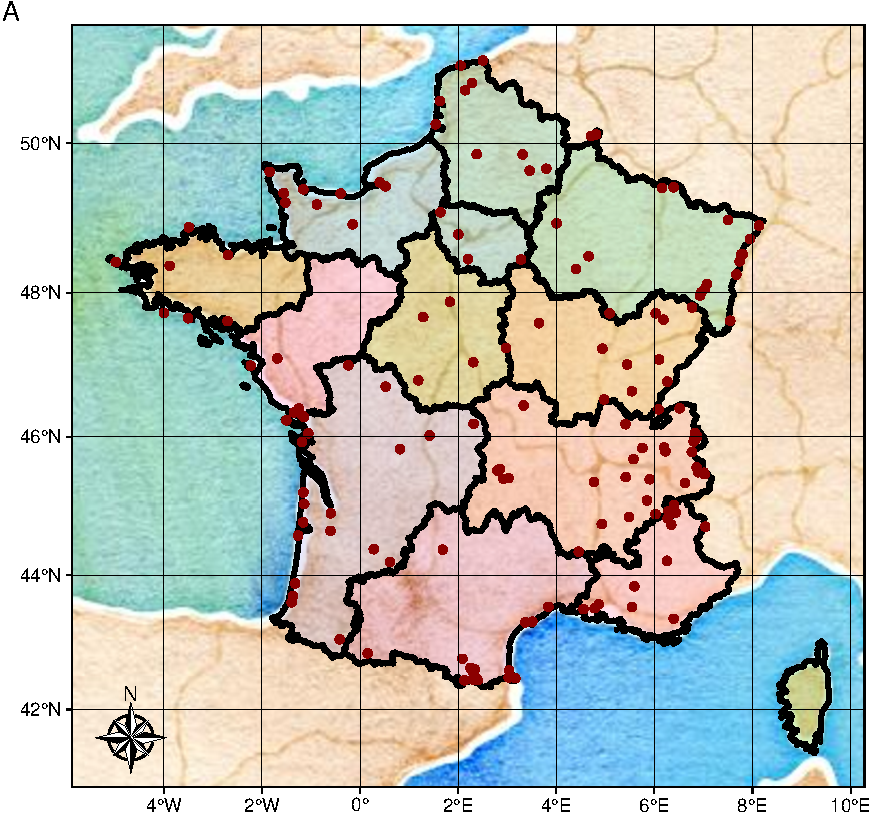
\includegraphics[width=1\linewidth]{Mon_aide_memoire_R_files/figure-latex/plot-rnn-1} 

}

\caption{Carte montrant la localisation géographique (point rouge) des Réserves Naturelles Nationales de la France métropolitaine. Un zoom a été fait pour apercevoir la délimitation de la Réserve Nationale de la Haute Chaîne du Jura.}\label{fig:plot-rnn}
\end{figure}

\hypertarget{rasters}{%
\subsection{Les rasters}\label{rasters}}

Un raster représente une image constituée de pixels (cellules) organisé(e)s sous
la forme d'une grille. C'est la représentation que l'on a l'habitude de voir
lorsque l'on parle d'une image numérique. Chaque pixel est unique et possède
certaines valeurs le caractérisant (comme sa couleur, ses coordonnées, son
altitude\ldots). Les données sont ainsi organisées en \textbf{matrice}, où chaque
\textbf{cellule} correspond à un pixel. Pour bien superposer le raster à la carte,
les matrices possèdent une en-tête incluant le \textbf{Système de Coordonnées de
Référence}, \textbf{l'origine} (généralement les coordonnées du coin inférieur droit
de la matrice), ainsi que l'\textbf{étendue de la matrice} (le nombre de colonnes, de
lignes et la résolution spatiale \footnote{Globalement, la résolution spatiale est la \textbf{taille réelle du
  plus petit élément} représenté dans un jeu de données. Pour le \emph{mode
  matriciel}, cela \textbf{correspond à la taille de la cellule de la grille}. Par
  exemple, si une cellule représente une surface réelle de 10 x 10 m, alors la
  résolution est de 10 m. La résolution spatiale permet donc de \textbf{définir le
  niveau de détail} du jeu de données. La netteté de l'image est ainsi dépendante
  de la résolution spatiale puisqu'il y aura plus de détails capturés avec des
  cellules de petite taille (résolution élevée ou fine) qu'avec des cellules de
  grande taille (résolution basse ou grossière).}).\\
De par leurs caractéristiques, les rasters permettent de définir des \textbf{données
discrètes} ainsi que des \textbf{données continues}.

\hypertarget{CRS}{%
\section{Les Systèmes de Coordonnées de Référence Géographiques et Projetées}\label{CRS}}

\begin{center}\rule{0.5\linewidth}{0.5pt}\end{center}

\hypertarget{ref-sig}{%
\section*{Liste de ressources Internet utiles}\label{ref-sig}}
\addcontentsline{toc}{section}{Liste de ressources Internet utiles}

\begin{itemize}
\tightlist
\item
  \href{https://geocompr.robinlovelace.net/}{Guide} sur les analyses de données
  géographiques, leur visualisation et leur modélisation sur R
\item
  \href{https://statnmap.com/2018-07-14-introduction-to-mapping-with-sf-and-co/}{Introduction}
  à l'utilisation des packages de cartographie sur R
\item
  \href{https://www.infoworld.com/article/3505897/how-to-do-spatial-analysis-in-r-with-sf.amp.html}{Introduction}
  au package \texttt{sf}
\item
  \href{https://github.com/r-spatial/mapedit}{Édition} interactive de cartes avec
  \texttt{mapedit}
\item
  \href{https://mhallwor.github.io/_pages/welcome}{introduction} à l'utilisation de R
  comme un SIG
\item
  \href{http://eriqande.github.io/rep-res-web/lectures/making-maps-with-R.html}{Introduction}
  pour créer des cartes avec R
\item
  \href{https://thinkr.fr/sil-te-plait-dessine-moi-carte-r/}{Introduction}
  en français pour créer des cartes avec R
\item
  Introduction en français sur le package
  \href{https://colinfay.me/carte-r-rgeoapi-ggplot2/}{\texttt{rgeoapi}}
\item
  \href{https://rgeomatic.hypotheses.org/tag/sf}{Zoomer} sur une carte avec R
\item
  \href{https://rpubs.com/huanfaChen/ggplotShapefile}{Tracer des cartes avec \texttt{ggplot2}}
  via des fichiers \emph{shapefiles}
\item
  \href{https://www.r-spatial.org/r/2018/10/25/ggplot2-sf.html}{Tutoriel}
  pour dessiner des cartes avec R, \texttt{sf} et \texttt{ggplot2}
\item
  \href{https://r-spatial.github.io/mapview/}{Cartes interactives} avec \texttt{mapview}
\item
  \href{https://rstudio.github.io/leaflet/}{Cartes interactives} avec \texttt{leaflet}
\item
  Guide pour faire des
  \href{https://www.tylermw.com/a-step-by-step-guide-to-making-3d-maps-with-satellite-imagery-in-r/}{cartes en 3D}
  à partir d'une imagerie satellite
\item
  Utilisation du package \href{https://www.rayshader.com/}{\texttt{rayshader}} pour la
  création de cartes en 2D et 3D
\item
  Manipulation et visualisation de données
  \href{https://github.com/Jean-Romain/lidR}{LiDAR} pour la foresterie avec \texttt{lidr}
\item
  \href{https://www.sigterritoires.fr/index.php/concepts/}{Blog français} contenant
  divers tutoriels sur la SIG et QGis
\item
  \href{https://naturagis.fr/}{NaturaGIS} : tutoriels et ressources sur la géomatique, les SIG et leurs usages pour l'environnement
\item
  \href{https://docs.qgis.org/3.10/fr/docs/}{Documentation officielle} de QGIS
\end{itemize}

\hypertarget{session-info}{%
\chapter*{Session info}\label{session-info}}
\addcontentsline{toc}{chapter}{Session info}

\begin{verbatim}
## - Session info ---------------------------------------------------------------
##  setting  value                       
##  version  R version 4.0.2 (2020-06-22)
##  os       Ubuntu 20.04.1 LTS          
##  system   x86_64, linux-gnu           
##  ui       X11                         
##  language (EN)                        
##  collate  fr_FR.UTF-8                 
##  ctype    fr_FR.UTF-8                 
##  tz       Europe/Paris                
##  date     2020-08-13                  
## 
## - Packages -------------------------------------------------------------------
##  package     * version    date       lib source                            
##  abind         1.4-5      2016-07-21 [1] CRAN (R 4.0.1)                    
##  assertthat    0.2.1      2019-03-21 [3] CRAN (R 4.0.0)                    
##  backports     1.1.8      2020-06-17 [3] CRAN (R 4.0.1)                    
##  bookdown      0.20       2020-06-23 [1] CRAN (R 4.0.2)                    
##  callr         3.4.3      2020-03-28 [3] CRAN (R 4.0.0)                    
##  class         7.3-17     2020-04-26 [4] CRAN (R 4.0.0)                    
##  classInt      0.4-3      2020-04-07 [1] CRAN (R 4.0.1)                    
##  cli           2.0.2      2020-02-28 [3] CRAN (R 4.0.0)                    
##  codetools     0.2-16     2018-12-24 [4] CRAN (R 4.0.0)                    
##  colorspace    1.4-1      2019-03-18 [3] CRAN (R 4.0.0)                    
##  crayon        1.3.4      2017-09-16 [3] CRAN (R 4.0.0)                    
##  DBI           1.1.0      2019-12-15 [1] CRAN (R 4.0.1)                    
##  desc          1.2.0      2018-05-01 [3] CRAN (R 4.0.0)                    
##  devtools      2.3.1      2020-07-21 [3] CRAN (R 4.0.2)                    
##  digest        0.6.25     2020-02-23 [3] CRAN (R 4.0.0)                    
##  dplyr       * 1.0.1      2020-07-31 [1] CRAN (R 4.0.2)                    
##  e1071         1.7-3      2019-11-26 [1] CRAN (R 4.0.1)                    
##  ellipsis      0.3.1      2020-05-15 [3] CRAN (R 4.0.0)                    
##  evaluate      0.14       2019-05-28 [3] CRAN (R 4.0.0)                    
##  fansi         0.4.1      2020-01-08 [3] CRAN (R 4.0.0)                    
##  farver        2.0.3      2020-01-16 [3] CRAN (R 4.0.0)                    
##  fs            1.5.0      2020-07-31 [3] CRAN (R 4.0.2)                    
##  generics      0.0.2      2018-11-29 [1] CRAN (R 4.0.1)                    
##  ggforce     * 0.3.2      2020-06-23 [1] CRAN (R 4.0.1)                    
##  ggplot2     * 3.3.2.9000 2020-08-11 [1] Github (tidyverse/ggplot2@6d91349)
##  ggrepel     * 0.9.0      2020-08-11 [1] Github (slowkow/ggrepel@4d0ef50)  
##  ggspatial   * 1.1.4      2020-07-12 [1] CRAN (R 4.0.2)                    
##  ggthemes    * 4.2.0      2019-05-13 [1] CRAN (R 4.0.1)                    
##  glue          1.4.1      2020-05-13 [3] CRAN (R 4.0.0)                    
##  gtable        0.3.0      2019-03-25 [3] CRAN (R 4.0.0)                    
##  highr         0.8        2019-03-20 [3] CRAN (R 4.0.0)                    
##  hms           0.5.3      2020-01-08 [1] CRAN (R 4.0.1)                    
##  htmltools     0.5.0      2020-06-16 [3] CRAN (R 4.0.1)                    
##  httr          1.4.2      2020-07-20 [3] CRAN (R 4.0.2)                    
##  jpeg          0.1-8.1    2019-10-24 [1] CRAN (R 4.0.1)                    
##  kableExtra    1.1.0      2019-03-16 [1] CRAN (R 4.0.1)                    
##  KernSmooth    2.23-17    2020-04-26 [4] CRAN (R 4.0.0)                    
##  knitr         1.29       2020-06-23 [1] CRAN (R 4.0.1)                    
##  lattice       0.20-41    2020-04-02 [4] CRAN (R 4.0.0)                    
##  lifecycle     0.2.0      2020-03-06 [3] CRAN (R 4.0.0)                    
##  magrittr      1.5        2014-11-22 [3] CRAN (R 4.0.0)                    
##  MASS          7.3-51.6   2020-04-26 [4] CRAN (R 4.0.0)                    
##  memoise       1.1.0      2017-04-21 [3] CRAN (R 4.0.0)                    
##  munsell       0.5.0      2018-06-12 [3] CRAN (R 4.0.0)                    
##  patchwork   * 1.0.1      2020-06-22 [1] CRAN (R 4.0.1)                    
##  pillar        1.4.6      2020-07-10 [3] CRAN (R 4.0.2)                    
##  pkgbuild      1.1.0      2020-07-13 [3] CRAN (R 4.0.2)                    
##  pkgconfig     2.0.3      2019-09-22 [3] CRAN (R 4.0.0)                    
##  pkgload       1.1.0      2020-05-29 [3] CRAN (R 4.0.0)                    
##  plyr          1.8.6      2020-03-03 [1] CRAN (R 4.0.1)                    
##  polyclip      1.10-0     2019-03-14 [1] CRAN (R 4.0.1)                    
##  prettymapr    0.2.2      2017-09-20 [1] CRAN (R 4.0.1)                    
##  prettyunits   1.1.1      2020-01-24 [3] CRAN (R 4.0.0)                    
##  processx      3.4.3      2020-07-05 [3] CRAN (R 4.0.2)                    
##  ps            1.3.4      2020-08-11 [1] CRAN (R 4.0.2)                    
##  purrr         0.3.4      2020-04-17 [3] CRAN (R 4.0.0)                    
##  R6            2.4.1      2019-11-12 [3] CRAN (R 4.0.0)                    
##  raster        3.3-13     2020-07-17 [1] CRAN (R 4.0.2)                    
##  Rcpp          1.0.5      2020-07-06 [3] CRAN (R 4.0.2)                    
##  readr         1.3.1      2018-12-21 [1] CRAN (R 4.0.1)                    
##  remotes       2.2.0      2020-07-21 [3] CRAN (R 4.0.2)                    
##  rgdal         1.5-16     2020-08-07 [1] CRAN (R 4.0.2)                    
##  rlang         0.4.7      2020-07-09 [1] CRAN (R 4.0.2)                    
##  rmarkdown     2.3.3      2020-07-31 [1] Github (rstudio/rmarkdown@204aa41)
##  rosm          0.2.5      2019-07-22 [1] CRAN (R 4.0.2)                    
##  rprojroot     1.3-2      2018-01-03 [3] CRAN (R 4.0.0)                    
##  rstudioapi    0.11       2020-02-07 [3] CRAN (R 4.0.0)                    
##  rvest         0.3.6      2020-07-25 [1] CRAN (R 4.0.2)                    
##  scales        1.1.1      2020-05-11 [3] CRAN (R 4.0.0)                    
##  sessioninfo   1.1.1      2018-11-05 [3] CRAN (R 4.0.0)                    
##  sf          * 0.9-5      2020-07-14 [1] CRAN (R 4.0.2)                    
##  sp            1.4-2      2020-05-20 [1] CRAN (R 4.0.2)                    
##  stringi       1.4.6      2020-02-17 [3] CRAN (R 4.0.0)                    
##  stringr       1.4.0      2019-02-10 [3] CRAN (R 4.0.0)                    
##  testthat      2.3.2      2020-03-02 [3] CRAN (R 4.0.0)                    
##  tibble        3.0.3      2020-07-10 [1] CRAN (R 4.0.2)                    
##  tidyselect    1.1.0      2020-05-11 [1] CRAN (R 4.0.1)                    
##  tweenr        1.0.1      2018-12-14 [1] CRAN (R 4.0.1)                    
##  units         0.6-7      2020-06-13 [1] CRAN (R 4.0.1)                    
##  usethis       1.6.1      2020-04-29 [3] CRAN (R 4.0.0)                    
##  vctrs         0.3.2      2020-07-15 [3] CRAN (R 4.0.2)                    
##  viridisLite   0.3.0      2018-02-01 [3] CRAN (R 4.0.0)                    
##  webshot       0.5.2      2019-11-22 [3] CRAN (R 4.0.0)                    
##  withr         2.2.0      2020-04-20 [3] CRAN (R 4.0.0)                    
##  xfun          0.16       2020-07-24 [1] CRAN (R 4.0.2)                    
##  xml2          1.3.2      2020-04-23 [3] CRAN (R 4.0.0)                    
##  yaml          2.2.1      2020-02-01 [3] CRAN (R 4.0.0)                    
## 
## [1] /home/alexis/R/x86_64-pc-linux-gnu-library/4.0
## [2] /usr/local/lib/R/site-library
## [3] /usr/lib/R/site-library
## [4] /usr/lib/R/library
\end{verbatim}

  \bibliography{book.bib,packages.bib}

\end{document}
